\chapter{Spécification et analyse des besoins
}
\fancyhead[R]{\textit{Spécification et analyse des besoins}}
\renewcommand{\headrulewidth}{1pt}


\section{Introduction}
Ce chapitre sera consacré à la phase de spécification et d’analyse des besoins.
dans cette étape, nous allons tout d’abord identifier les différents acteurs du
système, ainsi que leurs actions qui sont représentées en cas d’utilisation,
puis nous allons décrire les spécifications des exigences fonctionnelles et non
fonctionnelles, ainsi que leurs contraintes. Ceci nous permettra de modéliser le
diagramme de cas d’utilisation. 

\section{Identification des acteurs}
Un acteur représente une entité extérieure au système modélisé, qui interagit
directement avec lui afin d’atteindre des objectifs \cite{4}. Dans notre
système, on peut identifier 4 acteurs humains :
    
    
\begin{itemize}
    \item[\textbullet] \textbf{L’Employé :} Joue le rôle d’une personne qui
        occupe un emploi dans l’entreprise et qui interagit avec le système,
        pour un pointage des horaires de travail réalisé, ainsi que la
        possibilité de s’authentifier sur la plateforme pour consulter les
        informations qui le concernent.
    \item[\textbullet] \textbf{Le Manager :} Joue le rôle d’un employé très
        important qui est le lien entre la direction et les autres employés. Les
        managers s’occupent de l’organisation et du contrôle de leurs équipes et
        employés à travers la plateforme.
    \item[\textbullet] \textbf{Le Responsable :} Joue le rôle d’un responsable
        qui gère les employés ainsi que les différentes équipes de l’entreprise.
    \item[\textbullet] \textbf{L’administrateur :} Joue le rôle d’une personne
        vitale pour le bon fonctionnement du système via l’espace
        d’administration.
\end{itemize}
    
    
\section{Identifications des cas d'utilisation}
Un cas d’utilisation représente une série d’interactions d’un acteur avec un
système. Cette interaction est destinée à fournir des résultats à l’acteur. Le
tableau ci-dessous présente les différents cas d’utilisations avec leurs acteurs
respectifs.
    
\begin{longtable}{|c|c|c|c|}
    % header and footer information
     \endhead
     \endfoot
    % body of table
     \hline
     \textbf{N}& \multicolumn{2}{c|}{\textbf{Cas d’utilisation}} & \textbf{Acteur}\\
     \hline
     1 & \multicolumn{2}{c|} {S’authentifier} & \multirow{8}{*}{\shortstack{Employé/Manager\\ Responsable}} \\
     \cline{1-3}
     2 & \multicolumn{2}{c|} {Consulter mon tableau de bord} & 
     \\
     \cline{1-3}
     3 & \multicolumn{2}{c|} {Consulter ma fiche de pointage} &
     \\
     \cline{1-3}
     4 & \multicolumn{2}{c|} {Rechercher période} &
     \\
     \cline{1-3}
     5 & \multicolumn{2}{c|} {Consulter mon profile} &
     \\
     \cline{1-3}
     6 & \multicolumn{2}{c|} {Modifier mon profile} &
     \\
     \cline{1-3}
     7 & \multicolumn{2}{c|} {Consulter mon planning} &
     \\
     \cline{1-3}
     8 & \multicolumn{2}{c|} {Se pointer} & 
     \\
     \hline
     9 & \multicolumn{2}{c|} {Consulter tableau de bord manager} &
     \multirow{8}{*}{Manager}\\
     \cline{1-3}
     10 & \multicolumn{2}{c|} {Consulter liste des collaborateurs} &
     \\
     \cline{1-3}
     11 & \multicolumn{2}{c|} {Consulter profil d'un collaborateur} &
     \\
     \cline{1-3}
     12 & \multicolumn{2}{c|} {Consulter planning d'un collaborateur} &
     \\
     \cline{1-3}
     13 & \multicolumn{2}{c|} {Consulter liste de mes équipes} &
     \\
     \cline{1-3}
     14 & \multicolumn{2}{c|} {Consulter résumer de mon équipe} &
     \\
     \cline{1-3}
     15 & \multicolumn{2}{c|} {Consulter résumer de pointage des collaborateurs} &
     \\
     \cline{1-3}
     16 & \multicolumn{2}{c|} {Consulter feuille de pointage d’un collaborateurs} &
     \\
     \hline
     17 & \multicolumn{2}{c|} {Rechercher employé} &
     \multirow{1}{*}{Manager/Responsable}
     \\
     \hline
     18 & \multicolumn{2}{c|} {Consulter le tableau de bord responsable} & \multirow{10}{*}{Responsable}
     \\
     \cline{1-3}
     19 & \multicolumn{2}{c|} {Consulter liste des équipes} & 
     \\
     \cline{1-3}
     20 & \multicolumn{2}{c|} {Consulter résumer d’une équipe} & 
     \\
     \cline{1-3}
     21 & \multicolumn{2}{c|} {Consulter liste des employés} & 
     \\
     \cline{1-3}
     22 & \multicolumn{2}{c|} {Consulter profil d’un employé} & 
     \\
     \cline{1-3}
     23 & \multicolumn{2}{c|} {Consulter liste des plannings} & 
     \\
     \cline{1-3}
     24 & \multicolumn{2}{c|} {Consulter planning d'un employé} & \\
     \cline{1-3}
     25 & \multicolumn{2}{c|} {Consulter résumer de pointage des employés} & \\
     \cline{1-3}
     26 & \multicolumn{2}{c|} {Consulter feuille de pointage d’un employé} & \\
     \cline{1-3}
     27 & \multicolumn{2}{c|} {Consulter journal d'affectation} & \\
     \hline
     \multirow{4}{*}{28} & \multirow{4}{*}{Gérer les plannings}   &{Ajouter un planning} &  \\
     & & {Modifier un planning} & \\
     & & {Supprimer un planning} & \\
     & & {Affectation d'un planning} & \\
     \cline{1-3}
     \multirow{5}{*}{29} & \multirow{5}{*}{Gérer les équipes}   &{Ajouter une équipe} & \multirow{2}{*}{Responsable/Administrateur} \\
     & & {Modifier une équipe} & \\
     & & {Supprimer une équipe} & \\
     & & {Ajouter membre} & \\
     & & {Supprimer membre} & \\
     \hline
     30 & \multicolumn{2}{c|} {Importer/exporter} & \multirow{6}{*}{Responsable/Administrateur}  \\
     \cline{1-3}
     31 & \multicolumn{2}{c|} {Ajouter une empreinte} & \\
     \cline{1-3}
     32 & \multicolumn{2}{c|} {Supprimer une empreinte} & \\
     \cline{1-3}
     \multirow{3}{*}{33} & \multirow{3}{*}{Gérer les employés}   &{Ajouter un employé} & \\
     & & {Modifier un employé} & \\
     & & {Supprimer un employé} & \\
     \hline
\end{longtable}


\section{Spécification des exigences}

\subsection{Exigences fonctionnelles}
Les besoins fonctionnels expriment une action que doit effectuer le système en
réponse à une demande (sorties qui sont produites pour un ensemble donné
d’entrées). Par exemple, le système doit stocker les informations de pointage des
employés. Le système à concevoir devra répondre aux besoins que nous allons
citer. Afin de mettre en évidence les différentes informations accessibles selon
le rôle, nous avons décidé de les regrouper par acteur.

\begin{itemize}
    \item [\textbullet] \textbf{Employé :} Accès à son profil ainsi qu’aux
        informations de pointage et au planning qui le concerne, ainsi qu’aux
        informations publiques et aux statuts de présence des collaborateurs
        faisant partie de la même équipe que lui.
        
    \item [\textbullet] \textbf{Manager :} En plus des informations accessibles
        à l’employé, le manager doit avoir accès aux informations des équipes
        dont il est responsable ainsi qu’aux informations des membres qui les
        composent, aux plannings et aux informations de pointage y compris.

    \item [\textbullet] \textbf{Responsable :} Celui-ci doit avoir accès à la
        totalité des informations du système concernant tous les employés, quels
        que soient leurs statuts. Il doit être capable d’ajouter, modifier,
        supprimer des équipes ou des plannings, affecter un manager à une
        équipe, un planning à un employé, ajouter ou supprimer un employé à
        une équipe. Importer/exporter des informations de pointage est une
        fonctionnalité primordiale que doit avoir ce rôle.
        
    \item [\textbullet] \textbf{Administrateur :} La personne responsable de
        maintenir le système et de veiller à son bon fonctionnement a
        naturellement accès à l’espace d’administration du système à partir
        duquel elle pourra gérer les comptes des différents utilisateurs et leur
        assigner le bon rôle. En cas d’incohérences ou d’erreurs, ce dernier
        devrait avoir la possibilité d’intervenir de manière directe sur la base
        de données afin de résoudre ces cas. Ce dernier doit pouvoir aussi gérer
        les empreintes (ajout et suppression).
\end{itemize}

En plus des besoins précédemment cités, il existe des besoins partagés entre
tous les acteurs tels que :

\begin{itemize}
    \item [\textbullet] Authentification : Chaque utilisateur du futur système
        devrat être authentifié au préalable avec son nom d’utilisateur et son
        mot de passe avant tout accès à ce dernier. Le système devrait ensuite
        rediriger l’utilisateur vers son espace utilisateur qui varie selon son
        rôle.

    \item [\textbullet] Récupérations de mot de passe : Tous les utilisateurs
        pourront réinitialiser leurs mots de passe grâce à leurs adresses mail.
\end{itemize}
            
\subsection{Exigences non fonctionnelles}
Ce sont des besoins qui caractérisent le système, elles sont liées aux
contraintes pesant sur les fonctionnalités. La liste suivante représente les
besoins non fonctionnels de notre système :

\begin{itemize}
    \item [\textbullet] Performance : l’application doit assurer un temps de
        réponse minime, tout en répondant aux exigences de l’utilisateur.
    
    \item [\textbullet] Sécurité : aucune opération ne doit être possible sans
        authentification préalable. Une protection contre CSRF est impérative.
        Les informations doivent être accessibles aux utilisateurs possédant les
        bons droits d’accès seulement. Les mots de passe doivent être hashés
        puis stockés et jamais stockés en clair. Le système doit identifier la
        pointeuse afin d’accepter les informations reçues.
    
    \item [\textbullet] Ergonomie : les informations doivent êtres lisibles et
        facilement interprétables. Des graphiques résumant les informations
        pertinentes doivent être présentés à l’utilisateur. Une navigation
        simple et efficace. L’utilisation d’icônes explicites permettant de
        comprendre le sens des actions que l’utilisateur s’apprête à effectuer.
        Les actions critiques doivent toujours être confirmées avant leurs
        exécutions. Le système ne doit pas nécessiter une formation longue durée
        pour être utilisé, il doit offrir une prise en main rapide et facile
        sans beaucoup d’efforts.
    
     \item [\textbullet] Modularité du code : contenu du contexte et de la
         problématique traitée. On se doit de penser à l’évolution potentielle
         du système. Dans cette optique, il est primordial d’écrire un code
         lisible, modulaire et bien documenté pour faciliter la maintenance, la
         personnalisation, et l’évolutivité de la solution proposée.
\end{itemize}
                

\section{Diagramme des cas d'utilisation}
Les diagrammes de cas d’utilisation représentent la structure des
fonctionnalités nécessaires aux utilisateurs du système \cite{6}, nous allons
ici modéliser les diagrammes de cas d’utilisation des 4 acteurs du système pour
avoir une vue globale de ce dernier.

\clearpage  
\subsection{Diagramme de cas d'utilisation de l'employé}
    \begin{figure}[h!]
        \centering
        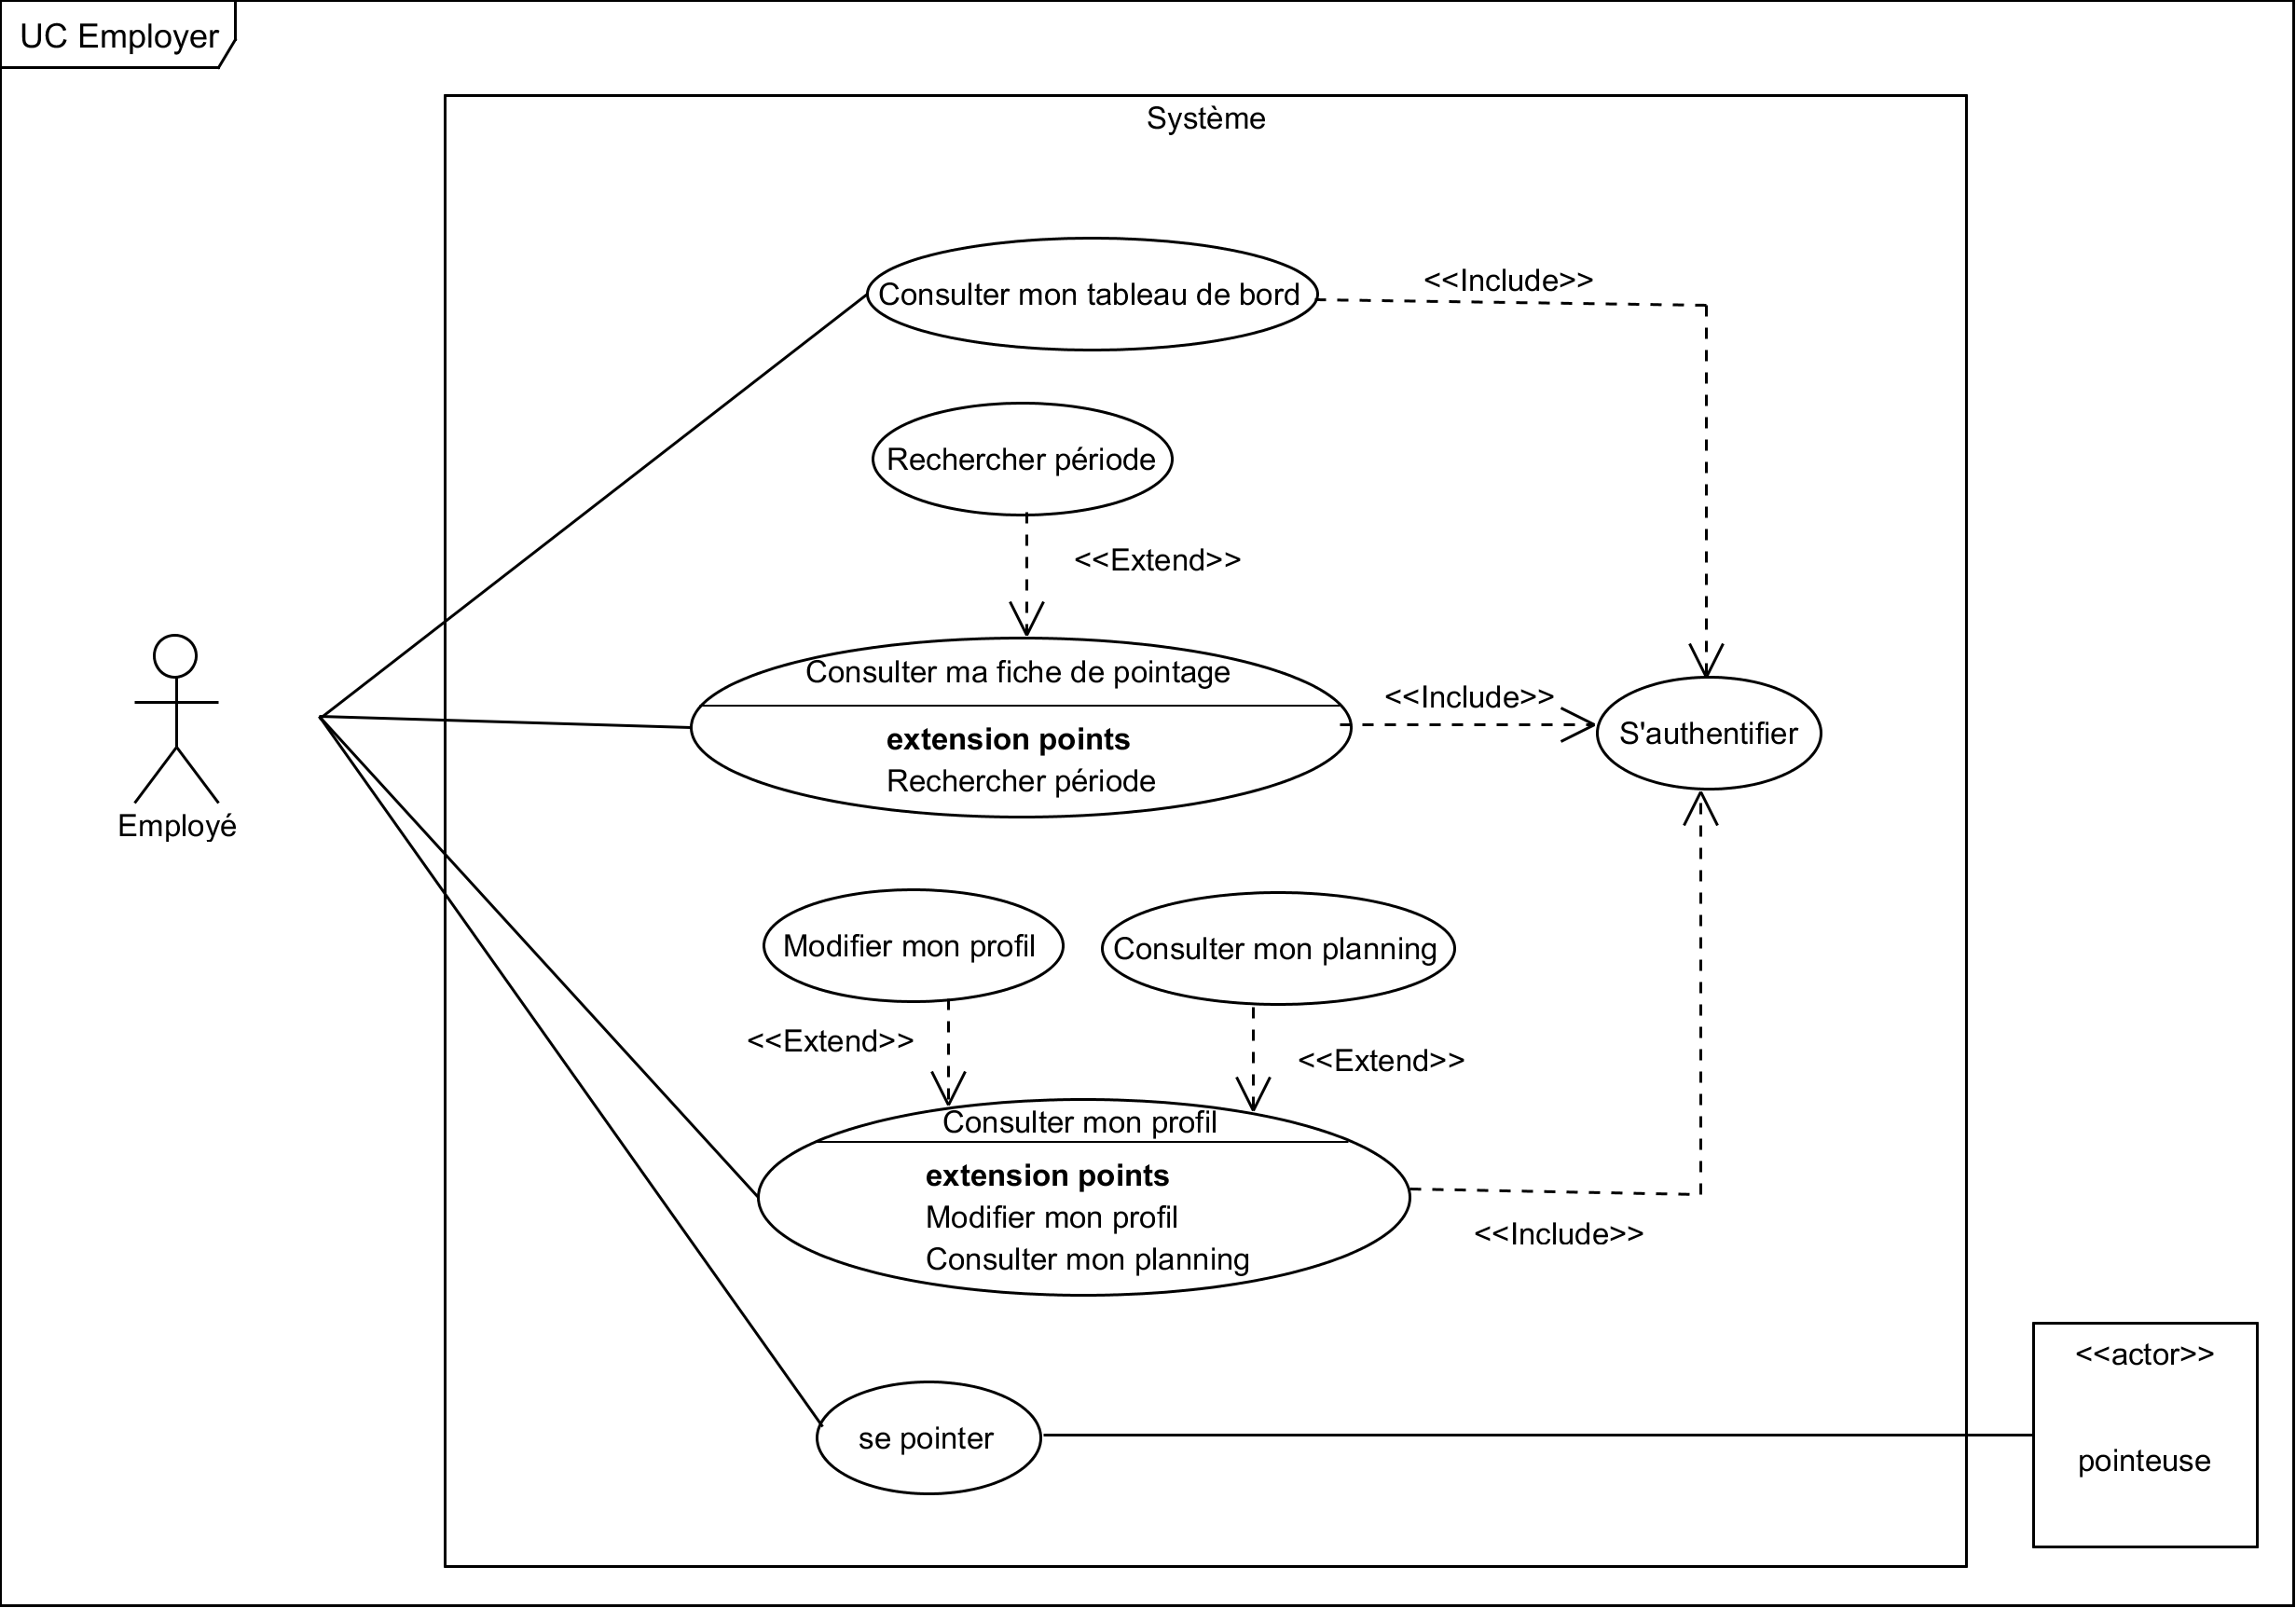
\includegraphics[angle=90, height=21cm]{images/uc_employe.png}
        \caption{Diagramme de cas d'utilisation associé à l'acteur «Employé»}
        \label{fig2}
    \end{figure}
    
\subsection{Diagramme de cas d'utilisation du manager}
    \begin{figure}[h!]
        \centering
        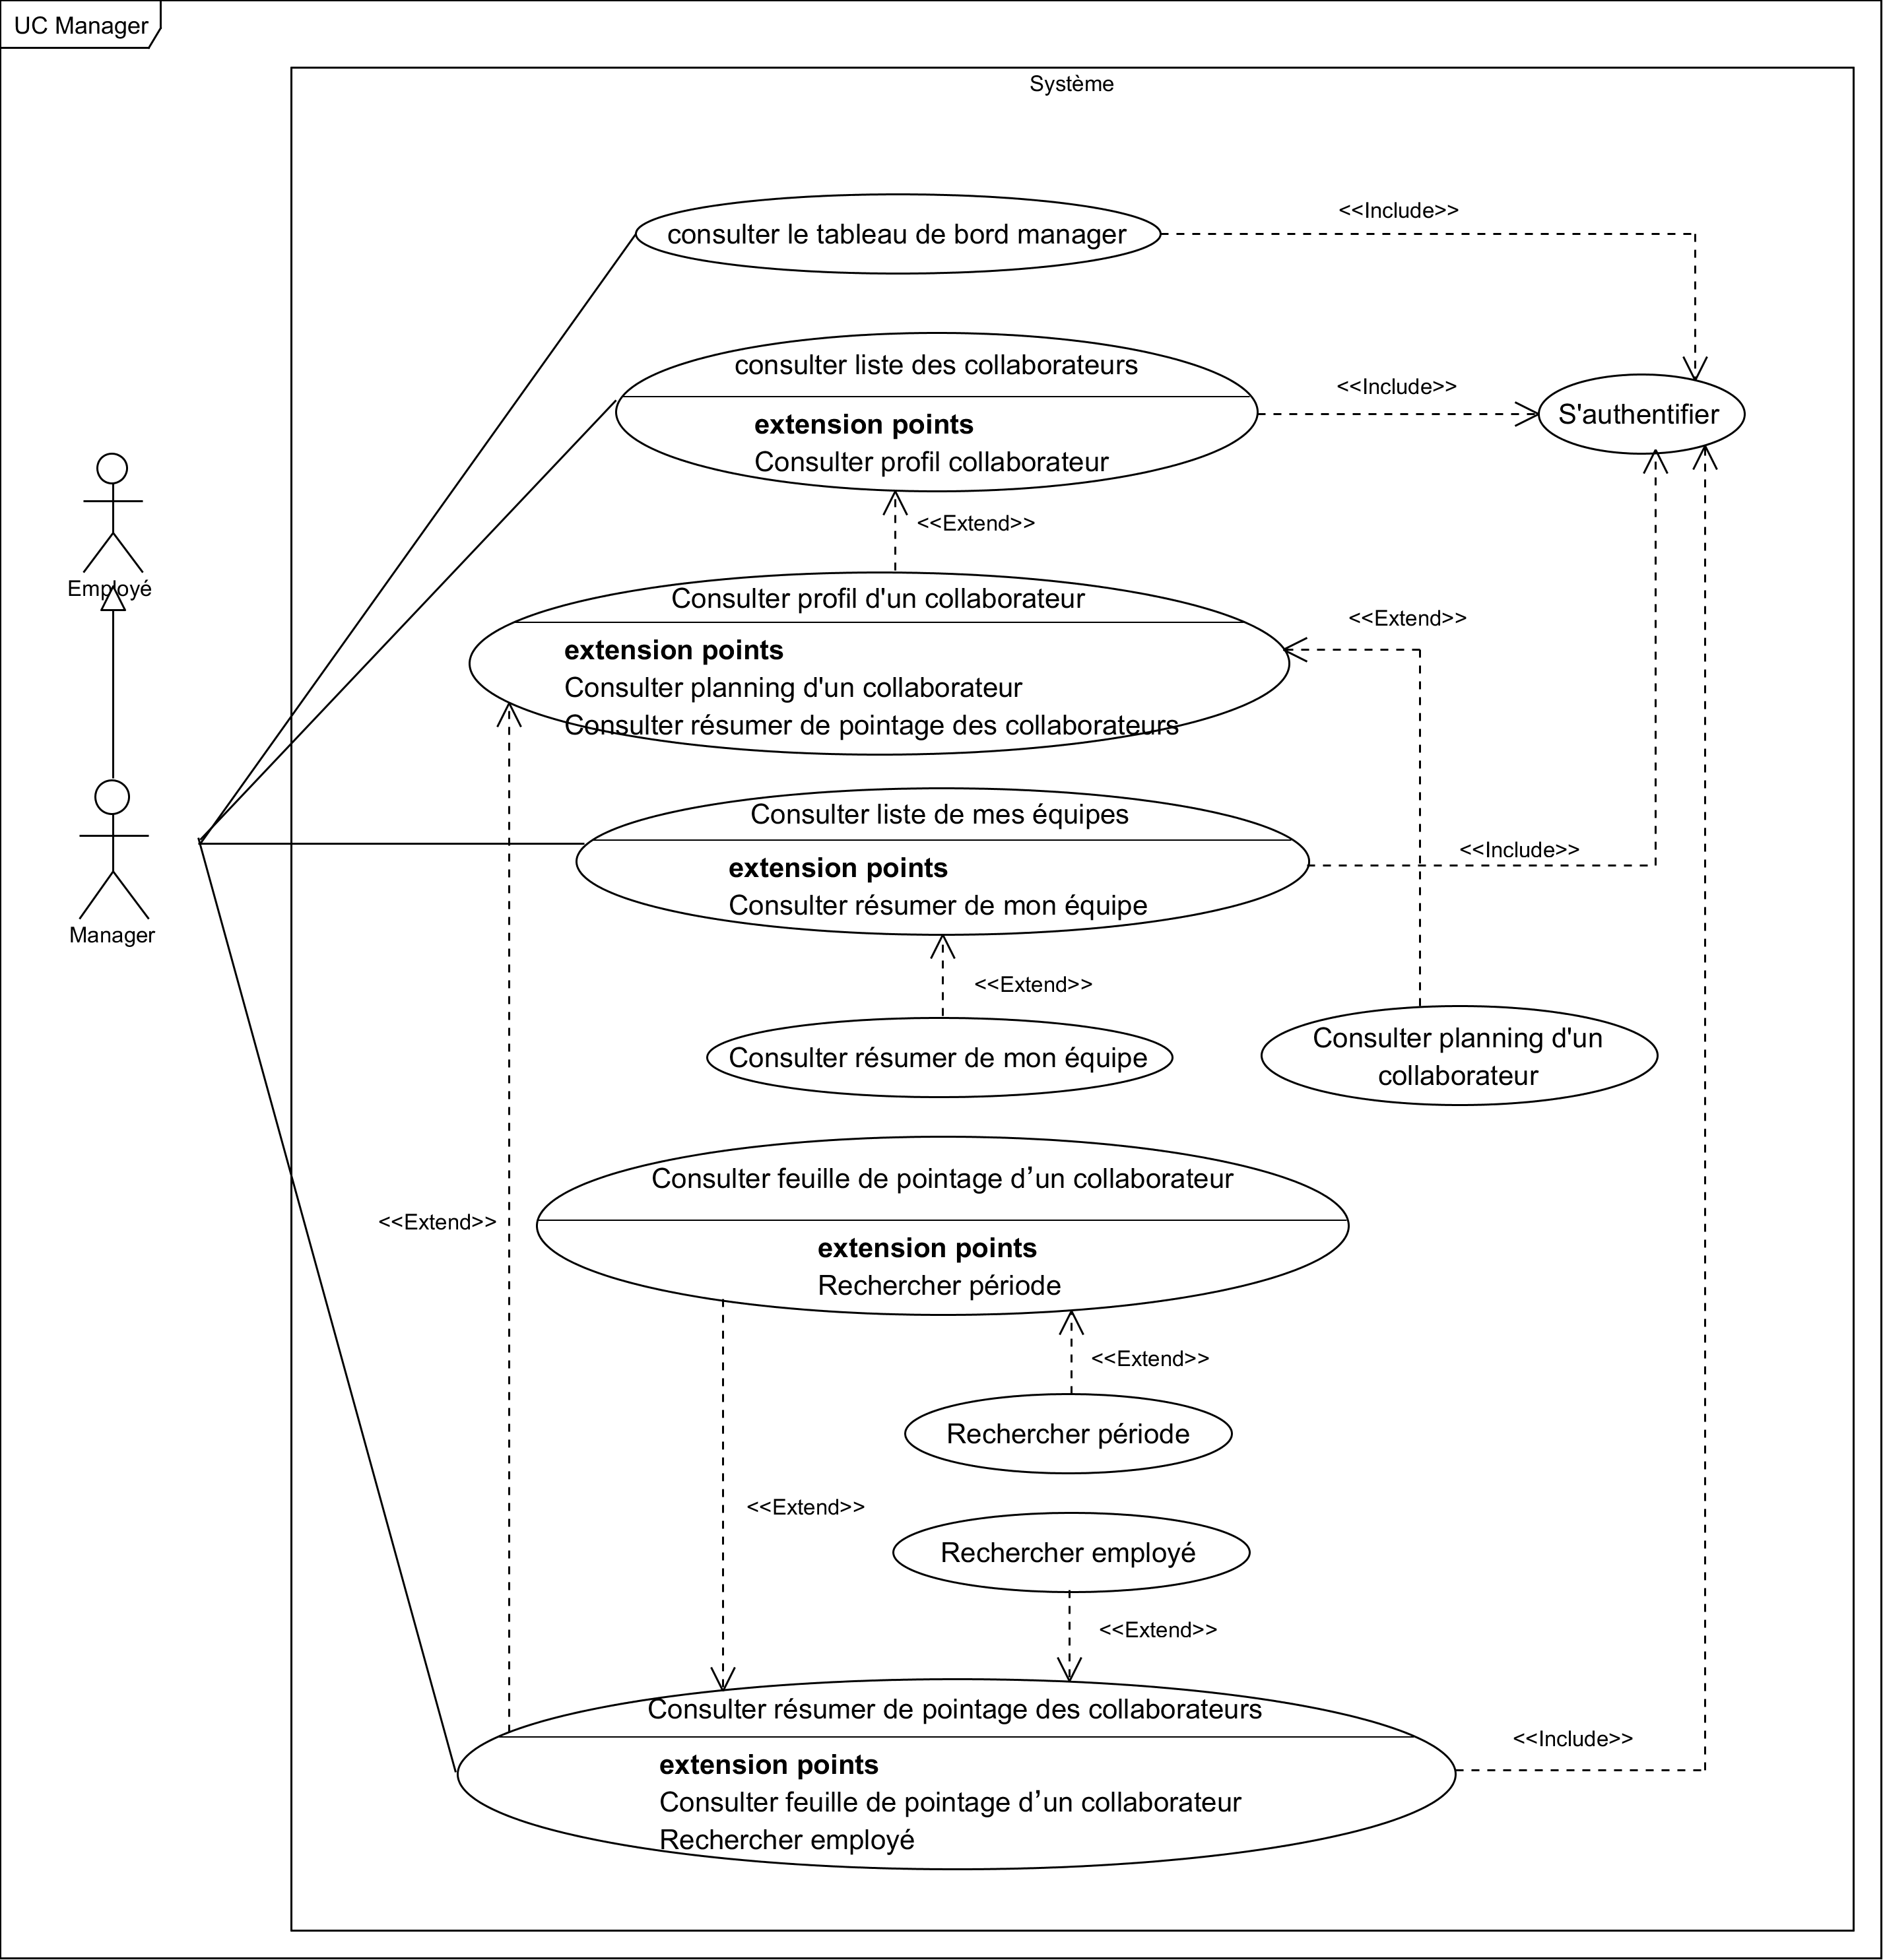
\includegraphics[width=16cm,height=21cm]{images/uc_manager.png}
        \caption{Diagramme de cas d'utilisation associé à l'acteur «Manager»}
        \label{fig3}
    \end{figure}

\clearpage  
 
\subsection{Diagramme de cas d'utilisation du responsable}
    \begin{figure}[h!]
         \centering
         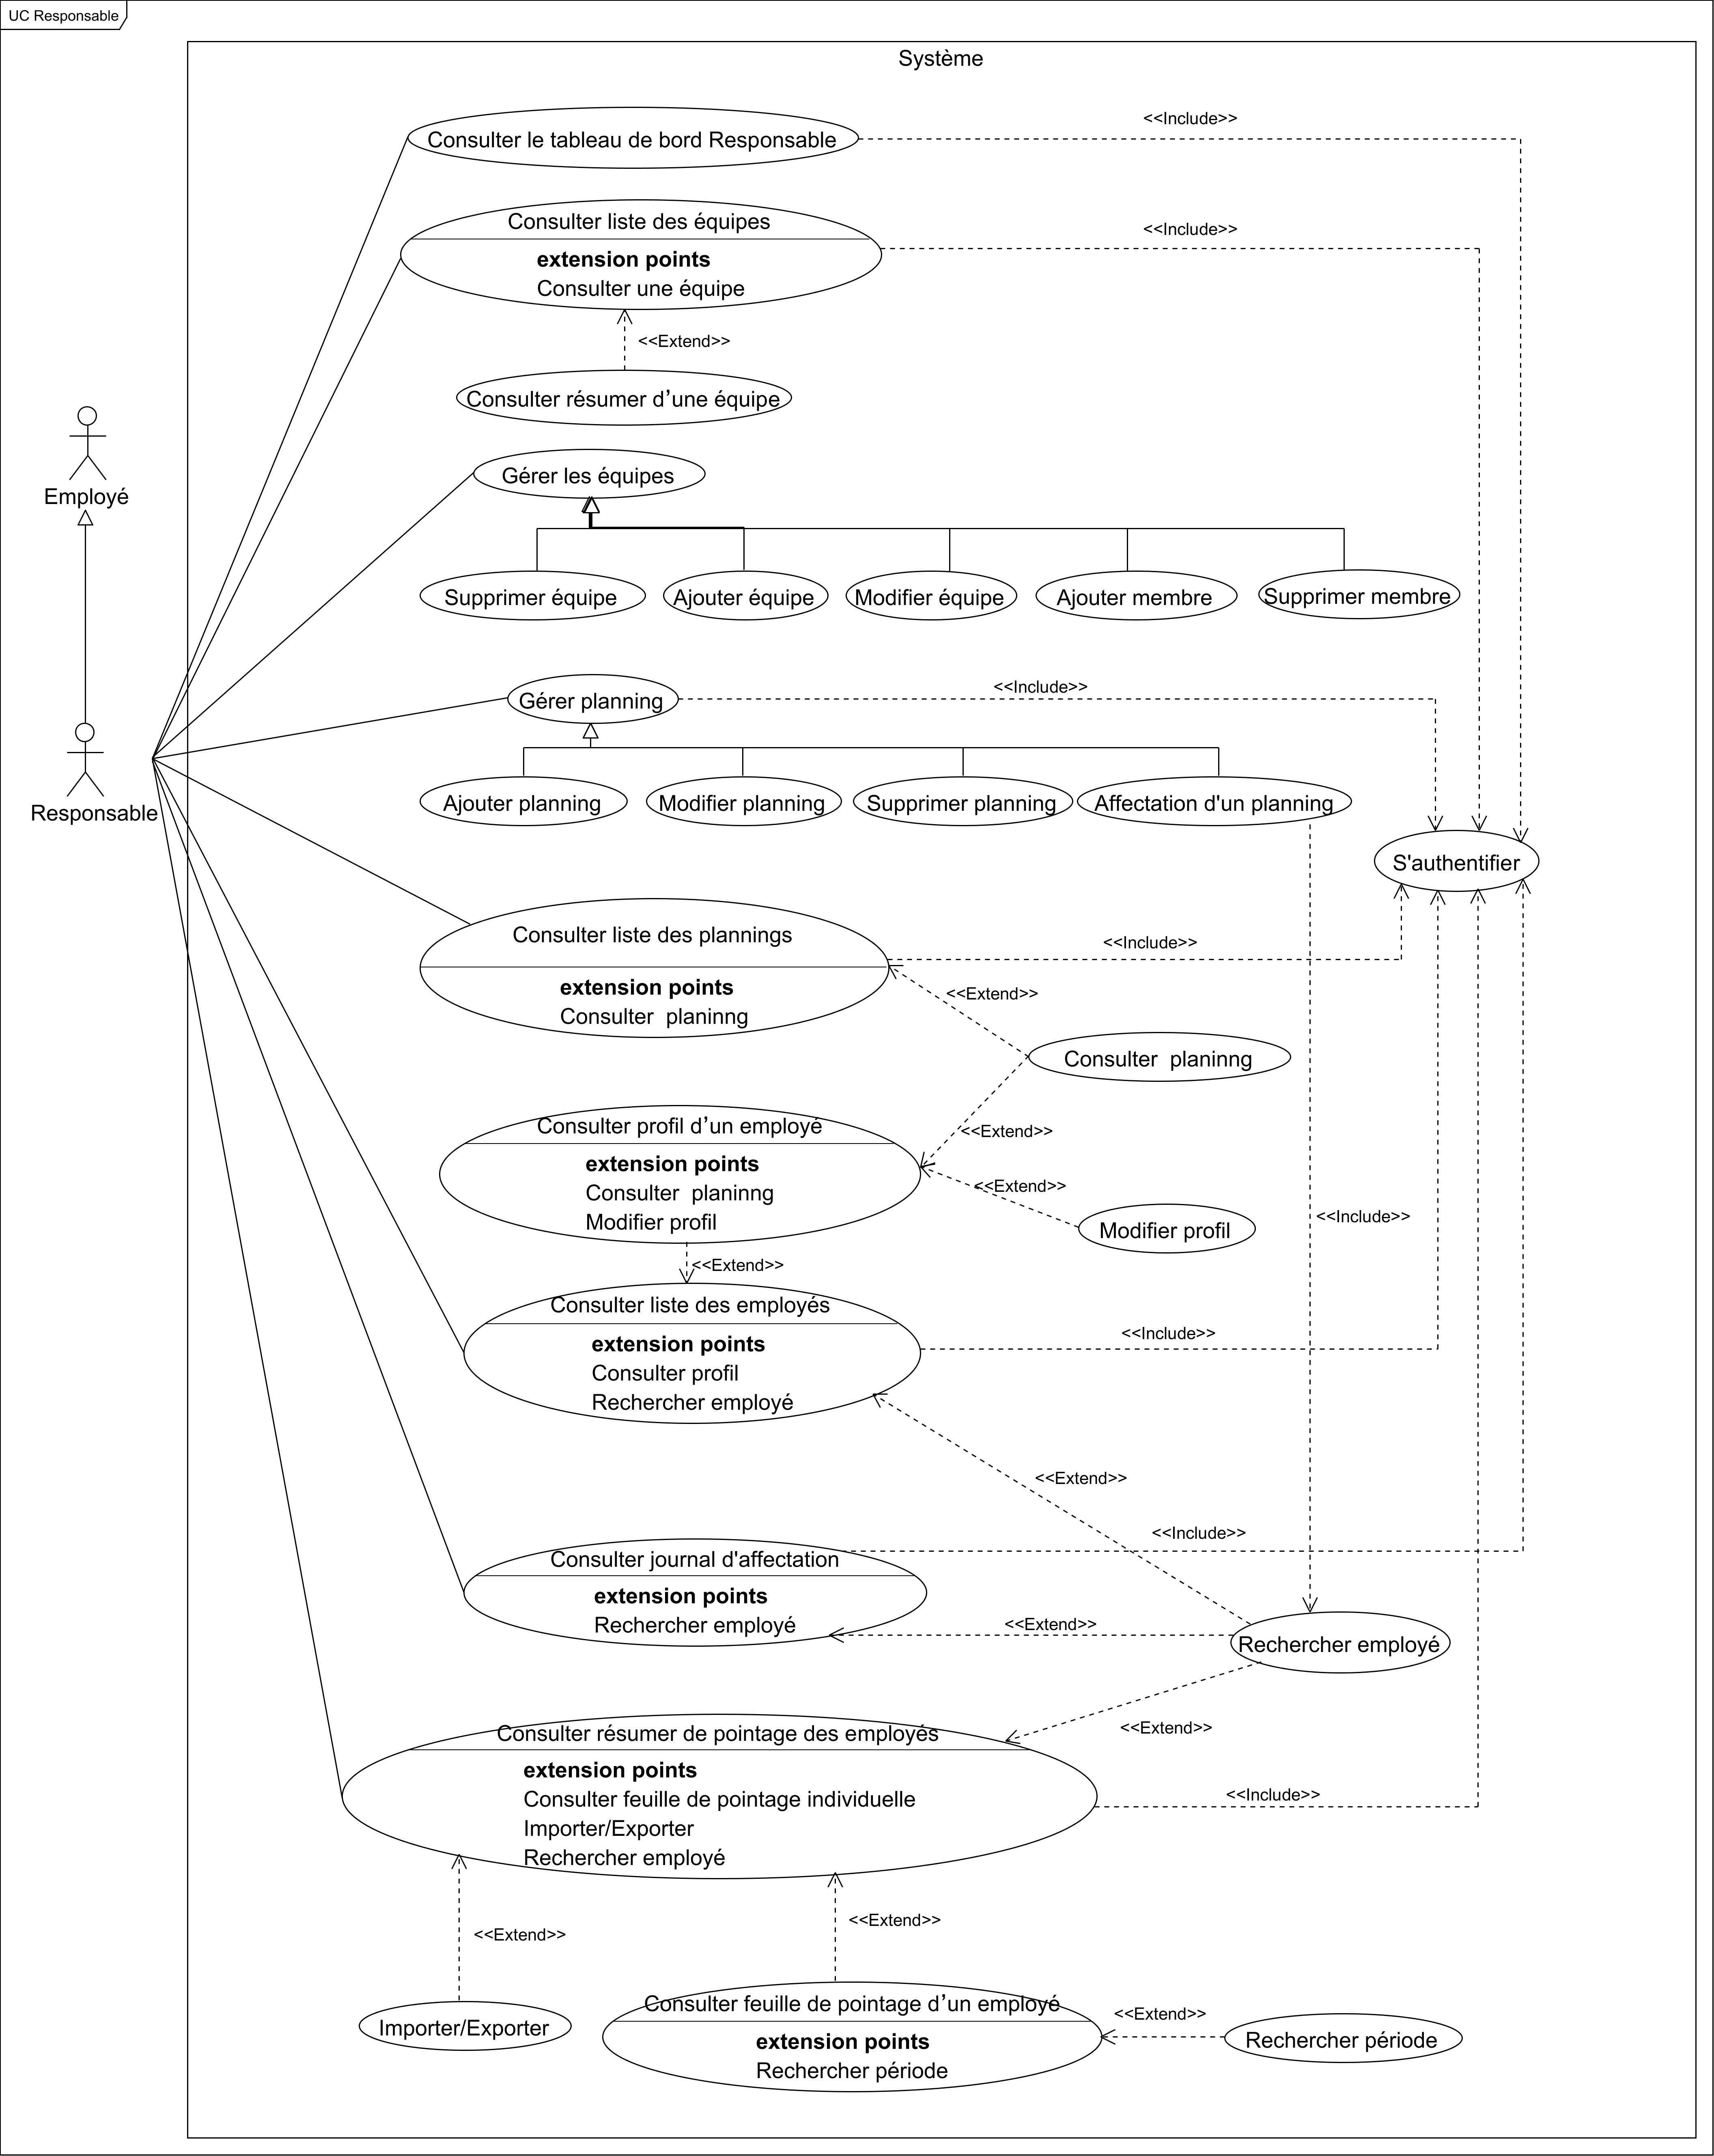
\includegraphics[width=17cm,height=21cm]{images/uc_responsable.png}
         \caption{Diagramme de cas d'utilisation associé à l'acteur «Responsable»}
         \label{fig4}
    \end{figure}
    
\clearpage  
 
\subsection{Diagramme de cas d'utilisation de l'administrateur}
    \begin{figure}[h!]
         \centering
         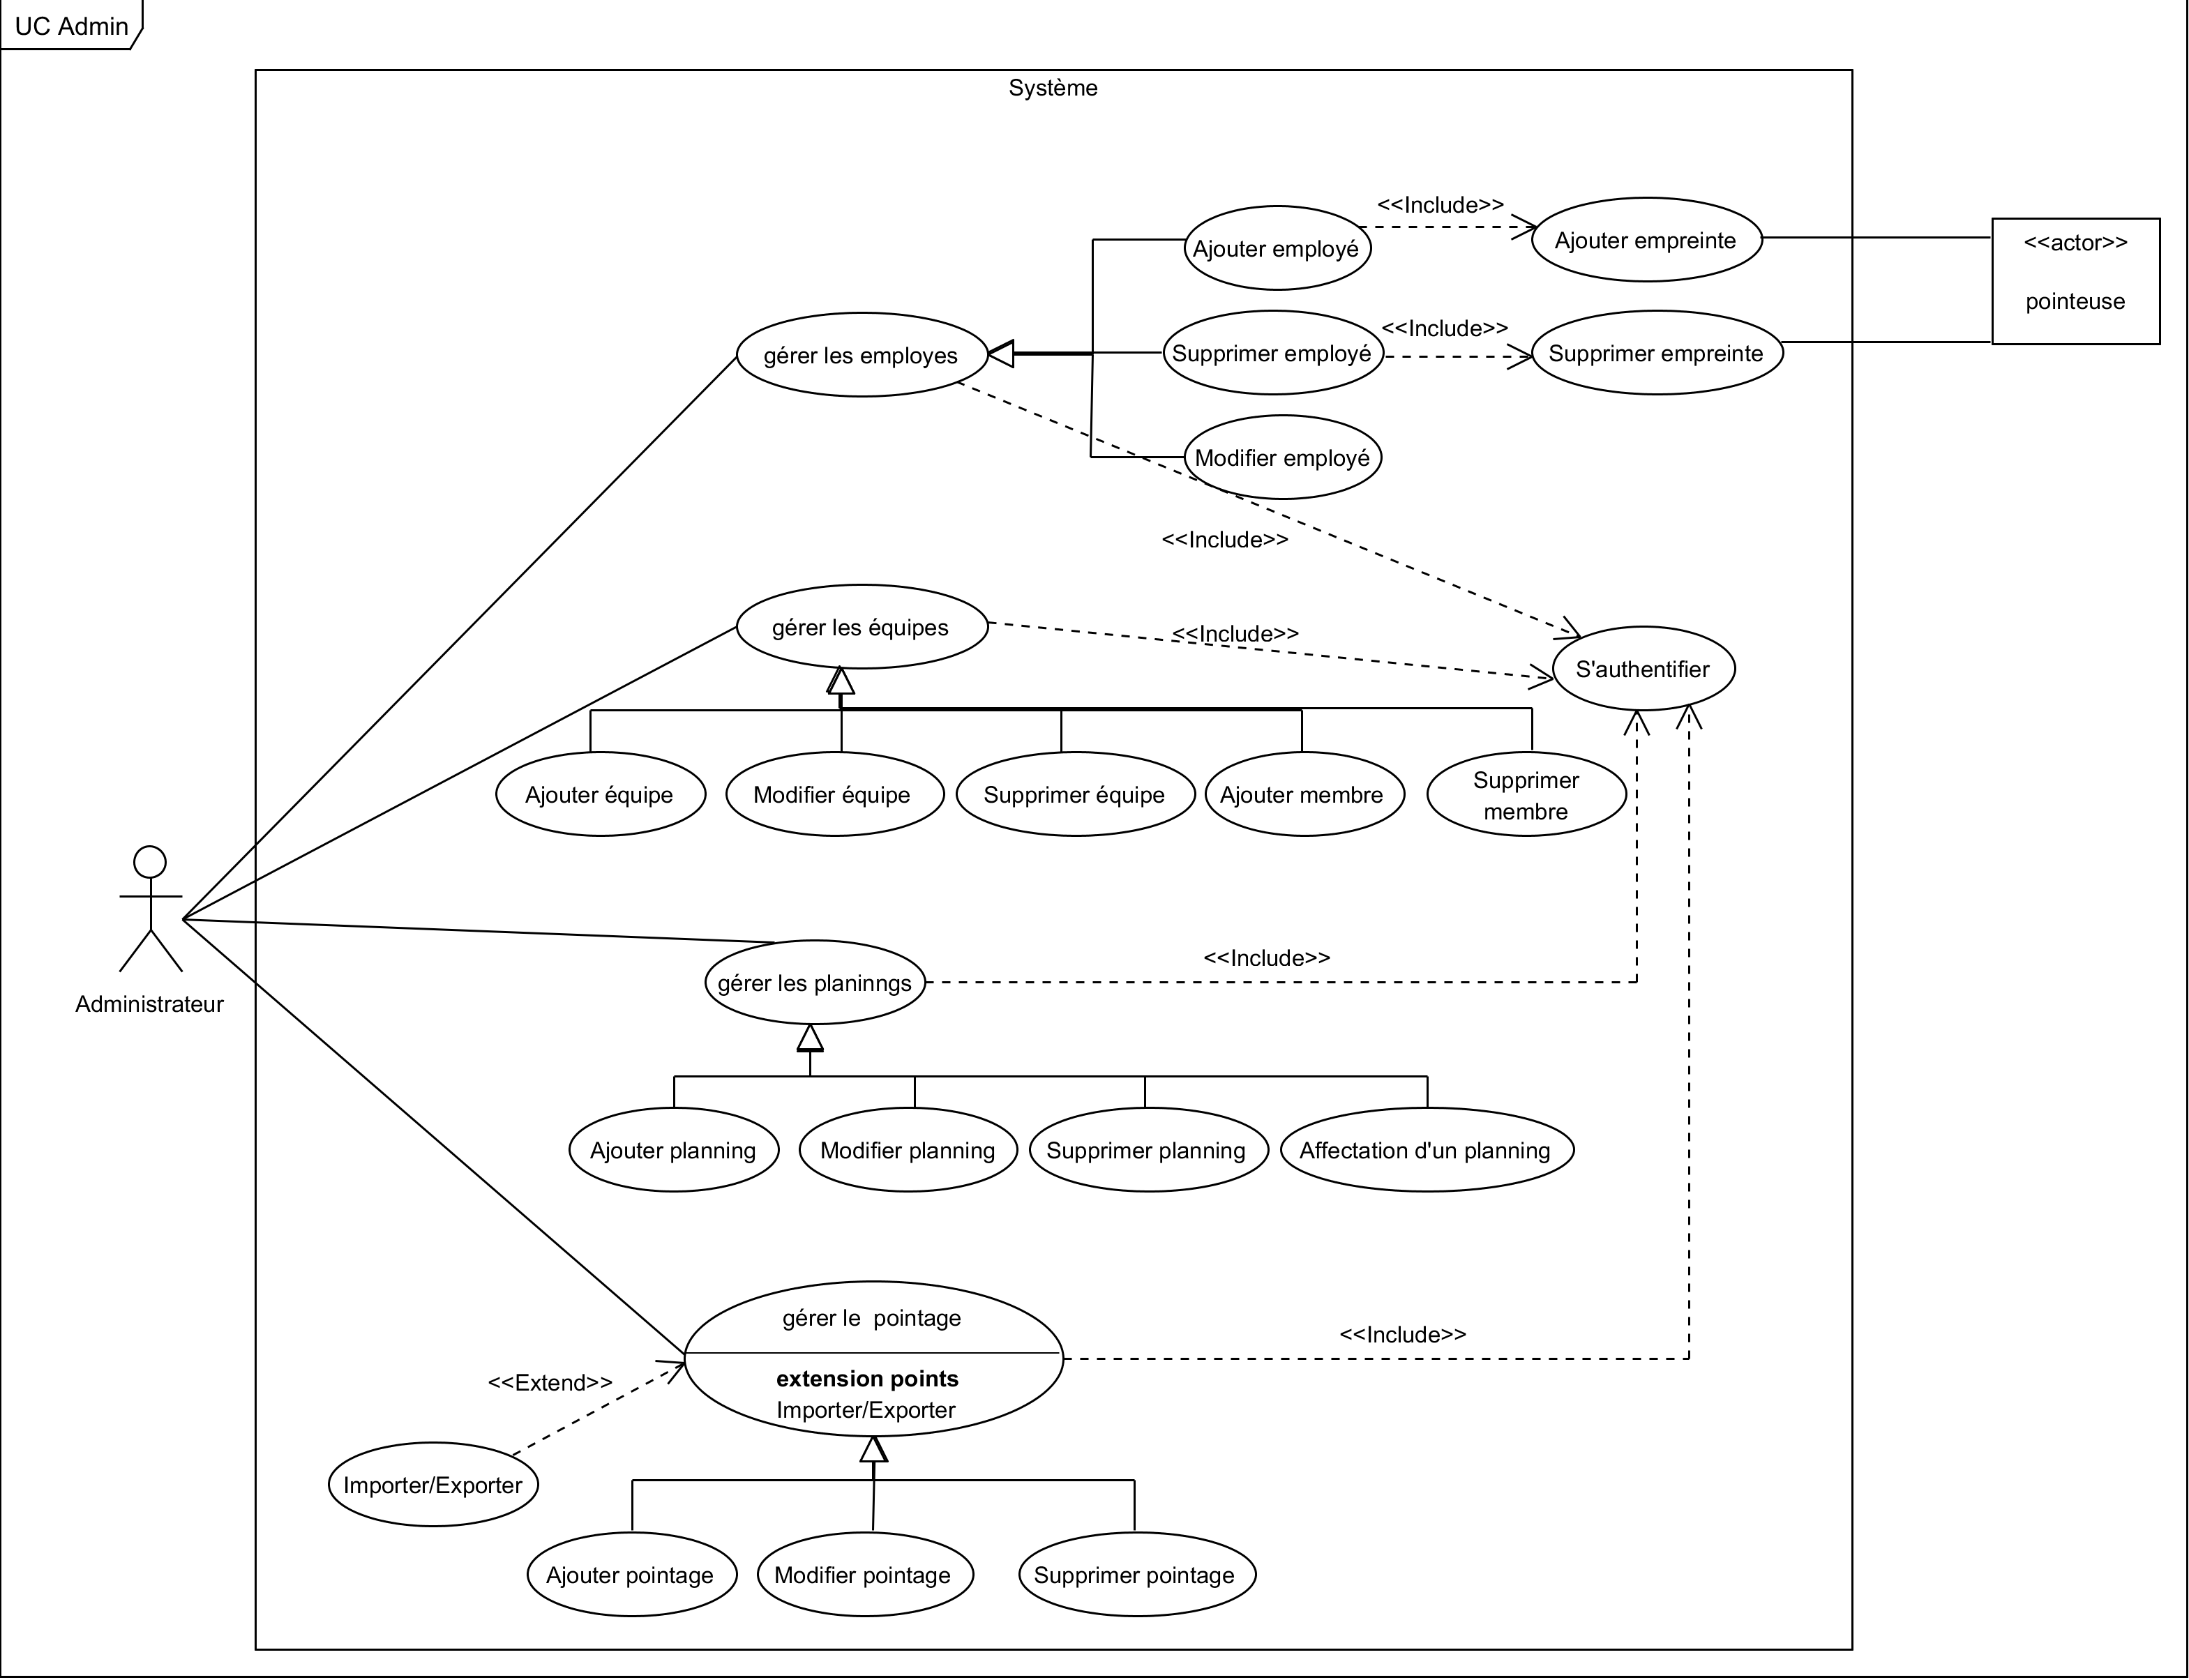
\includegraphics[angle=90, height=21cm]{images/uc_admin.png}
         \caption{Diagramme de cas d'utilisation associé à l'acteur «Administrateur»}
         \label{fig5}
    \end{figure}

\clearpage
\textcolor{red}{
L’objectif de certains cas d’utilisation est même en surface néanmoins ils sont
exécutés par des acteurs différents et dans des champs d’action distincts. On
peut illustrer ça avec le cas d’utilisation « Consulter mon profil », «
Consulter profil d’un collaborateur » et « Consulter profil d’un employé ». 
}

Le premier cas concerne un employé qui consulte son propre profil en ayant la
possibilité de modifier certaines informations. Le deuxième cas est déclenché
par le manager pour consulter le profil d’un collaborateur sans pouvoir le
modifier. Le troisième est utilisé par un administrateur pour consulter le
profil d’un employé (quel que soit son rôle) avec la possibilité de modifier
toutes les informations. 

\section{Descriptions de cas d'utilisation}
Les cas d’utilisation ne représentent pas uniquement les interactions avec les
acteurs, mais ils ajoutent également les prés et post conditions ainsi que les
enchaînements alternatifs. Dans cette partie, nous allons décrire les diagrammes
de cas d’utilisation des différents acteurs.
    
\subsection*{Cas d'utilisation « S'authentifier »}

\begin{longtable}{|p{4cm}|p{12cm}|}
    % header and footer information
    \endhead
    \endfoot
    % body of table
    \hline
    \multicolumn{2}{|c|}{\textbf{Sommaire d’identification}} \\
    \hline
    Titre & \textbf{S'authentifier} \\
    \hline
    Acteur & Employé, Manager, Responsable, Administrateur \\
    \hline
    Résumer & L’acteur doit s’identifier en saisissant son nom d'utilisateur et mot de passe pour accéder a son espace personnel. \\
    \hline
    \multicolumn{2}{|c|}{Description des scénarios} \\
    \hline
    Pré-conditions &  L’utilisateur doit être créé par l'administrateur. \\
    \hline
    Scénario nominal &  
    \begin{minipage}[t]{\linewidth}
        \begin{enumerate}[itemindent=0pt, leftmargin=*, nosep,before=\vspace{-0.5\baselineskip}]
            \item Le système affiche le formulaire d'authentification.
            \item L'acteur saisit le nom d'utilisateur ainsi que son mot de passe.
            \item Le système vérifie si les identifiants saisis sont corrects.
            \item Le système affiche le tableau de bord (voir le cas d’utilisations « Consulter mon tableau de bord »)
        \end{enumerate}
    \end{minipage}
    \\
    \hline
    Enchaînement alternatif &  
    \begin{minipage}[t]{\linewidth}
        2a. Les identifiants saisis par l'acteur sont incorrects.
        \begin{enumerate}[nosep,after=\strut]
            \item Le système affiche un message d'erreur pour signaler que les identifiants sont incorrects.
            \item Le cas d’utilisation reprend de l’étape 1 du scénario nominale.
        \end{enumerate}
    \end{minipage}
    \hline
    Postconditions & L'utilisateur est authentfié et accède aux fonctionnalités qui lui sont dédiées.  \\
    \hline
    \caption{Description du cas d'utilisation « S'authentifier »}\\
\end{longtable}

\subsection*{Cas d'utilisation « Se pointer »}
\begin{longtable}{|p{4cm}|p{12cm}|}
    % header and footer information
    \endhead
    \endfoot
    % body of table
    \hline
    \multicolumn{2}{|c|}{\textbf{Sommaire d’identification}} \\
    \hline
    Titre & \textbf{Se pointer} \\
    \hline
    Acteur & Employé, Manager, Responsable, Pointeuse  \\
    \hline
    Résumer & Un acteur signale son entrée ou sa sortie de l'entreprise en posant son index sur la pointeuse. \\
    \hline
    \multicolumn{2}{|c|}{Description des scénarios} \\
    \hline
    Pré-conditions & Être enregistrer dans le système (empreinte et profile)  \\
    \hline
    Scénario nominal &   

    \begin{minipage}[t]{\linewidth}
        \begin{enumerate}[itemindent=0pt, leftmargin=*, nosep,before=\vspace{-0.5\baselineskip}]
            \item L’acteur pose son index sur le lecteur d'empreinte.
            \item La pointeuse reconnait l’acteur et envoie un signal au système.
            \item Le système accuse la réception du signal.
            \item La pointeuse reçoit un accusé de réception et fait clignoter une LED, pour signaler le bon déroulement de l’opération de pointage.
        \end{enumerate}
    \end{minipage}
    \\
    \hline
    Enchaînement alternatif &   
    \begin{minipage}[t]{\linewidth}
        2a La pointeuse ne reconnait pas l’acteur.
        \begin{enumerate}[nosep,after=\strut]
            \item La LED de la pointeuse ne clignotera pas.
            \item Le cas d’utilisation reprend de l’étape 1 du scénario nominale.
        \end{enumerate}
    \end{minipage}
    \\
    \hline
    Postconditions &  Le système enregistrent l’heure et l’ID de l’employé responsable de l’événement. \\
    \hline
    Postconditions &   \\
    \hline
    \caption{Description du cas d'utilisation « Se pointer »}\\
\end{longtable}        
        
\subsection*{Cas d'utilisation « Consulter mon profil »}
\begin{longtable}{|p{4cm}|p{12cm}|}
    % header and footer information
    \endhead
    \endfoot
    % body of table
    \hline
    \multicolumn{2}{|c|}{\textbf{Sommaire d’identification}} \\
     \hline
     Titre & \textbf{Consulter mon profil} \\
     \hline
        Acteur & Employé, Manager, Responsable \\
        \hline
        Résumer & L’acteur accède aux informations qui constitue son profile. \\
        \hline
        \multicolumn{2}{|c|}{Description des scénarios} \\
        \hline
        Pré-conditions &  Être authentifier. \\
        \hline
        Scénario nominal & 
        \begin{minipage}[t]{\linewidth} \begin{enumerate}[itemindent=0pt, leftmargin=*, nosep,after=\vspace{-\baselineskip},before=\vspace{-0.5\baselineskip}]
            \item Les différentes informations du profile son afficher.
        \end{enumerate}
        \end{minipage}
         \\
        \hline
        Enchaînement alternatif &  
        1a. L’employé peut modifier ses informations (voir le cas d’utilisations « modifier mon profile »)
        \\
        
        \hline
        Postconditions &   \\
        \hline
        \caption{Description du cas d'utilisation « Consulter mon profil »}\\
\end{longtable}        
        
\subsection*{Cas d'utilisation « Consulter ma fiche de pointage »}
\begin{longtable}{|p{4cm}|p{12cm}|}
        % header and footer information
        \endhead
        \endfoot
        % body of table
        \hline
         \multicolumn{2}{|c|}{\textbf{Sommaire d’identification}} \\
         \hline
         Titre & \textbf{Consulter ma fiche de pointage} \\
         \hline
            Acteur & Employé, Manager, Responsable \\
            \hline
            Résumer &  L’acteur accède aux informations relatives à son pointage (Heures d’arrivée et de sortie) \\
            \hline
            \multicolumn{2}{|c|}{Description des scénarios} \\
            \hline
            Pré-conditions & Être authentifier.  \\
            \hline
            Scénario nominal &  
            \begin{minipage}[t]{\linewidth}
                \begin{enumerate}[itemindent=0pt, leftmargin=*, nosep,after=\vspace{-\baselineskip},before=\vspace{-0.5\baselineskip}]
                      \item Le système affiche les informations de pointage de l’acteur concerné pour une semaine.
                      \\\\
                      
                \end{enumerate}
            \end{minipage}
            \\
            \hline
            Enchaînement alternatif & 
            \begin{minipage}[t]{\linewidth}
                1a. l'acteur choisi d'avoir un affichage par mois.
                \begin{enumerate}[nosep,after=\strut]
                      \item Le système affiche les informations de pointage de l’acteur concerné pour un mois.
                \end{enumerate}
            \end{minipage}
            \\
            
            \hline
            Postconditions &   \\
            \hline
        \caption{Description du cas d'utilisation « Consulter ma fiche de pointage »}\\
\end{longtable}
            
\subsection*{Cas d'utilisation « Consulter tableau de bord manager »}
\begin{longtable}{|p{4cm}|p{12cm}|}
    % header and footer information
    \endhead
    \endfoot
    % body of table
    \hline
     \multicolumn{2}{|c|}{\textbf{Sommaire d’identification}} \\
     \hline
     Titre & \textbf{Consulter tableau de bord manager} \\
     \hline
        Acteur & Manager \\
        \hline
        Résumer & Le manager consulte son tableau de bord, qui est constitué de deux parties.La première représente le tableau de bord du manager en tan que employé tendis que la deuxième qui est un récapitulatif des informations de pointage de son/ses équipes et de tous ses collaborateurs). \\
        \hline
        \multicolumn{2}{|c|}{Description des scénarios} \\
        \hline
        Pré-conditions &  Le manager doit être authentifié. \\
        \hline
        Scénario nominal &  
            \begin{minipage}[t]{\linewidth}
                \begin{enumerate}[itemindent=0pt, leftmargin=*, nosep,before=\vspace{-0.5\baselineskip}]
                      \item Le système affiche un résumé des informations de pointage concernant le manager et son planning du jour.
                \end{enumerate}
            \end{minipage}
        \\
        \hline
        Enchaînement alternatif & 
            \begin{minipage}[t]{\linewidth}
            1a. Le manager décide de consulter la deuxième partie de son tableau de bord.
             \begin{enumerate}[nosep,after=\strut]
                      \item Le système affiche la partie qui concerne ses équipes ainsi que les collaborateurs encadrés par le manager en question.
                \end{enumerate}
            \end{minipage}
        \\
        
        \hline
        Postconditions &   \\
        \hline
    \caption{Description du cas d'utilisation « Consulter tableau de bord manager »}\\
\end{longtable}        
        
\subsection*{Cas d'utilisation « Ajouter membre »}
\begin{longtable}{|p{4cm}|p{12cm}|}
    % header and footer information
    \endhead
    \endfoot
    % body of table
    \hline
    \multicolumn{2}{|c|}{\textbf{Sommaire d’identification}} \\
     \hline
     Titre & \textbf{Ajouter membre} \\
     \hline
        Acteur & Responsable, Administrateur \\
        \hline
        Résumer & L’acteur accède à une interface qui lui permet d'affecter des employés à l'équipe'. \\
        \hline
        \multicolumn{2}{|c|}{Description des scénarios} \\
        \hline
        Pré-conditions &  Être authentifier. \\
        \hline
        Scénario nominal & 
        \begin{minipage}[t]{\linewidth} \begin{enumerate}[itemindent=0pt, leftmargin=*, nosep,after=\vspace{-\baselineskip},before=\vspace{-0.5\baselineskip}]
            \item L'acteur recherche un employé (voir le cas d’utilisations \underline{Recherche employé }).
            \item Le système retourne une liste d'employés.
            \item L'acteur sélectionne un employé et l'ajoute.
            \item Le système affiche l'interface d'affectation avec les données mise à jour.\\\\
        \end{enumerate}
        \end{minipage}
         \\
        \hline
        Enchaînement alternatif &  
        \begin{minipage}[t]{\linewidth}
            2a. Aucun employé trouver. \begin{enumerate}[nosep,after=\strut]
                  \item Le système affiche un message d'erreur.
            \end{enumerate}
        \end{minipage}
        \\
        
        \hline
        Postconditions &   \\
        \hline
        \caption{Description du cas d'utilisation « Ajouter membre »}\\
\end{longtable}        
        
\subsection*{Cas d'utilisation « Ajouter un planning »}  
\begin{longtable}{|p{4cm}|p{12cm}|}
        % header and footer information
        \endhead
        \endfoot
        % body of table
        \hline
        \multicolumn{2}{|c|}{\textbf{Sommaire d’identification}} \\
         \hline
         Titre & \textbf{Ajouter équipe} \\
         \hline
            Acteur & Responsable, Administrateur \\
            \hline
            Résumer & L’acteur accède à une interface qui lui permet la création d'un nouveau planning. \\
            \hline
            \multicolumn{2}{|c|}{Description des scénarios} \\
            \hline
            Pré-conditions &  Être authentifier. \\
            \hline
            Scénario nominal & 
            \begin{minipage}[t]{\linewidth} \begin{enumerate}[itemindent=0pt, leftmargin=*, nosep,after=\vspace{-\baselineskip},before=\vspace{-0.5\baselineskip}]
                \item Le système affiche le formulaire.
                \item L'acteur saisit le nom du planning ainsi que la description et les horaires de travail.
                \item Le système vérifie la conformité des informations saisie.
                \item Le système affiche la liste des plannings voir cas d'utilisations \underline{ Consulter liste des plannings}.\\\\
            \end{enumerate}
            \end{minipage}
             \\
            \hline
            Enchaînement alternatif &  
            \begin{minipage}[t]{\linewidth}
                2a. Le nom de l'équipe est déjà existant.
                \begin{enumerate}[nosep,after=\strut]
                      \item Le système affiche un message d'erreur pour signaler que le nom du planning existe dans la base de données.
                      \item Le cas d’utilisation reprend de l’étape 1 du scénario nominale.
                \end{enumerate}
            \end{minipage}
            \\
            
            \hline
            Postconditions &   \\
            \hline
            \caption{Description du cas d'utilisation « Ajouter un planning »}\\
\end{longtable}        
        
\subsection*{Cas d'utilisation « Ajouter équipe »}  
    \begin{longtable}{|p{4cm}|p{12cm}|}
            % header and footer information
            \endhead
            \endfoot
            % body of table
            \hline
            \multicolumn{2}{|c|}{\textbf{Sommaire d’identification}} \\
             \hline
             Titre & \textbf{Ajouter équipe} \\
             \hline
                Acteur & Responsable, Administrateur \\
                \hline
                Résumer & L’acteur accède à une interface qui lui permet la création d'une nouvelle équipe. \\
                \hline
                \multicolumn{2}{|c|}{Description des scénarios} \\
                \hline
                Pré-conditions &  Être authentifier. \\
                \hline
                Scénario nominal & 
                \begin{minipage}[t]{\linewidth} \begin{enumerate}[itemindent=0pt, leftmargin=*, nosep,after=\vspace{-\baselineskip},before=\vspace{-0.5\baselineskip}]
                    \item Le système affiche le formulaire.
                    \item L'acteur saisit le nom de l'équipe ainsi que la description et sélectionne le manager de cette dernière.
                    \item Le système vérifie la conformité des informations saisie.
                    \item Le système affiche l'interface d'affectation des membres de l'équipe (voir le cas d’utilisations « affectation des membres »).\\\\
                \end{enumerate}
                \end{minipage}
                 \\
                \hline
                Enchaînement alternatif &  
                \begin{minipage}[t]{\linewidth}
                    2a. Le nom de l'équipe est déjà existant.
                    \begin{enumerate}[nosep,after=\strut]
                          \item Le système affiche un message d'erreur pour signaler que le nom de l'équipe existe dans la base de données.
                          \item Le cas d’utilisation reprend de l’étape 1 du scénario nominale.
                    \end{enumerate}
                \end{minipage}
                \\
                
                \hline
                Postconditions &   \\
                \hline
                \caption{Description du cas d'utilisation « Ajouter équipe »}\\
        \end{longtable}        
        
\subsection*{Cas d'utilisation « Ajouter un employé  »}
        \begin{longtable}{|p{4cm}|p{12cm}|}
            % header and footer information
            \endhead
            \endfoot
            % body of table
            \hline
            \multicolumn{2}{|c|}{\textbf{Sommaire d’identification}} \\
            \hline
            Titre & \textbf{Ajouter un employé} \\
             \hline
                Acteur &  Administrateur\\
                \hline
                Résumer &  L’administrateur ajoute un employé.\\
                \hline
                \multicolumn{2}{|c|}{Description des scénarios} \\
                \hline
                Pré-conditions &  Être authentifier   \\
                \hline
                Scénario nominal &  
                \begin{minipage}[t]{\linewidth}
                        \begin{enumerate}[itemindent=0pt, leftmargin=*, nosep,before=\vspace{-0.5\baselineskip},after=\vspace{0.2\baselineskip}]
                            \item L’administrateur saisit l’ensemble des informations de l’employé.
                            \item L’administrateur enregistre l’employé.
                            \item L’administrateur enregistre l’empreinte de l’employé (Cas d’utilisation \underline{Ajouter une empreinte}).
                        \end{enumerate}
                \end{minipage}
                \\
                \hline
                Enchaînement alternatif & 
                \begin{minipage}[t]{\linewidth}
                        2a Les informations saisies ne sont pas valides.
                        \begin{enumerate}[nosep,after=\strut, leftmargin=*]
                            \item Le système affiche un message qui spécifie les informations incorrectes et demande au responsable de les corriger.
                            \item Le cas d’utilisation reprend de l’étape 1 du scénario nominal.
                        \end{enumerate}
                \end{minipage}
                \\
                
                \hline
                Postconditions & Mise à jour des données présentes dans la base de données.
                \\
                \hline
                \caption{Description du cas d'utilisation « Ajouter un employé »}\\
        \end{longtable}        
        
\subsection*{Cas d'utilisation « Consulter profil d'un employé »}
        \begin{longtable}{|p{4cm}|p{12cm}|}
            % header and footer information
            \endhead
            \endfoot
            % body of table
            \hline
                 \multicolumn{2}{|c|}{\textbf{Sommaire d’identification}} \\
                 \hline
                 Titre & \textbf{Consulter profil d'un employé} \\
                 \hline
                    Acteur & Responsable \\
                    \hline
                    Résumer & Le responsable consulte le profil d’un employé. \\
                    \hline
                    \multicolumn{2}{|c|}{Description des scénarios} \\
                    \hline
                    Pré-conditions &  Le responsable doit être authentifié. \\
                    \hline
                    Scénario nominal &  
                        \begin{minipage}[t]{\linewidth}
                            \begin{enumerate}[itemindent=0pt, leftmargin=*, nosep,before=\vspace{-0.5\baselineskip},after=\vspace{0.2\baselineskip}]
                                \item L’acteur sélectionne un employé (Cas d’utilisation \underline{Consulter liste des employés}).
                                \item Le système affiche le profil de l'employé sélectionner.
                                \item L'acteur peut modifier le profil (Cas d’utilisation \underline{Modifier profil}).
                            \end{enumerate}
                        \end{minipage}
                    \\
                    \hline
                    Enchaînement alternatif & 
                        
                    \\
                    
                    \hline
                    Postconditions &   \\
                    \hline
                \hline
                \caption{Description du cas d'utilisation « Consulter profil d'un employé »}\\
        \end{longtable}        
        
            
Nous avons établi la totalité des descriptions des cas d’utilisation, mais nous
avons décidé de ne pas inclure tous des tableaux afin de ne pas encombrer le
lecteur. Néanmoins, le reste des descriptions est cité dans l’annexe A.
\ref{ch:annexeA}.  
    
                
\section{Diagramme de séquence système DSS}
Nous utilisons le terme de diagramme de séquence « système » pour souligner le
fait que nous considérons le système informatique comme une boîte noire, nous
ouvrirons la boîte noire seulement en conception.\cite{5}
    
\subsection{Cas d'utilisation « Se pointer »}
L’employé doit marquer ses heures de travails via la pointeuse biométrique, qui
vérifie son empreinte puis enregistre son pointage et lui signal le bon
déroulement de l’opération en allumant une LED.

\clearpage
    \begin{figure}[h!]
         \centering
        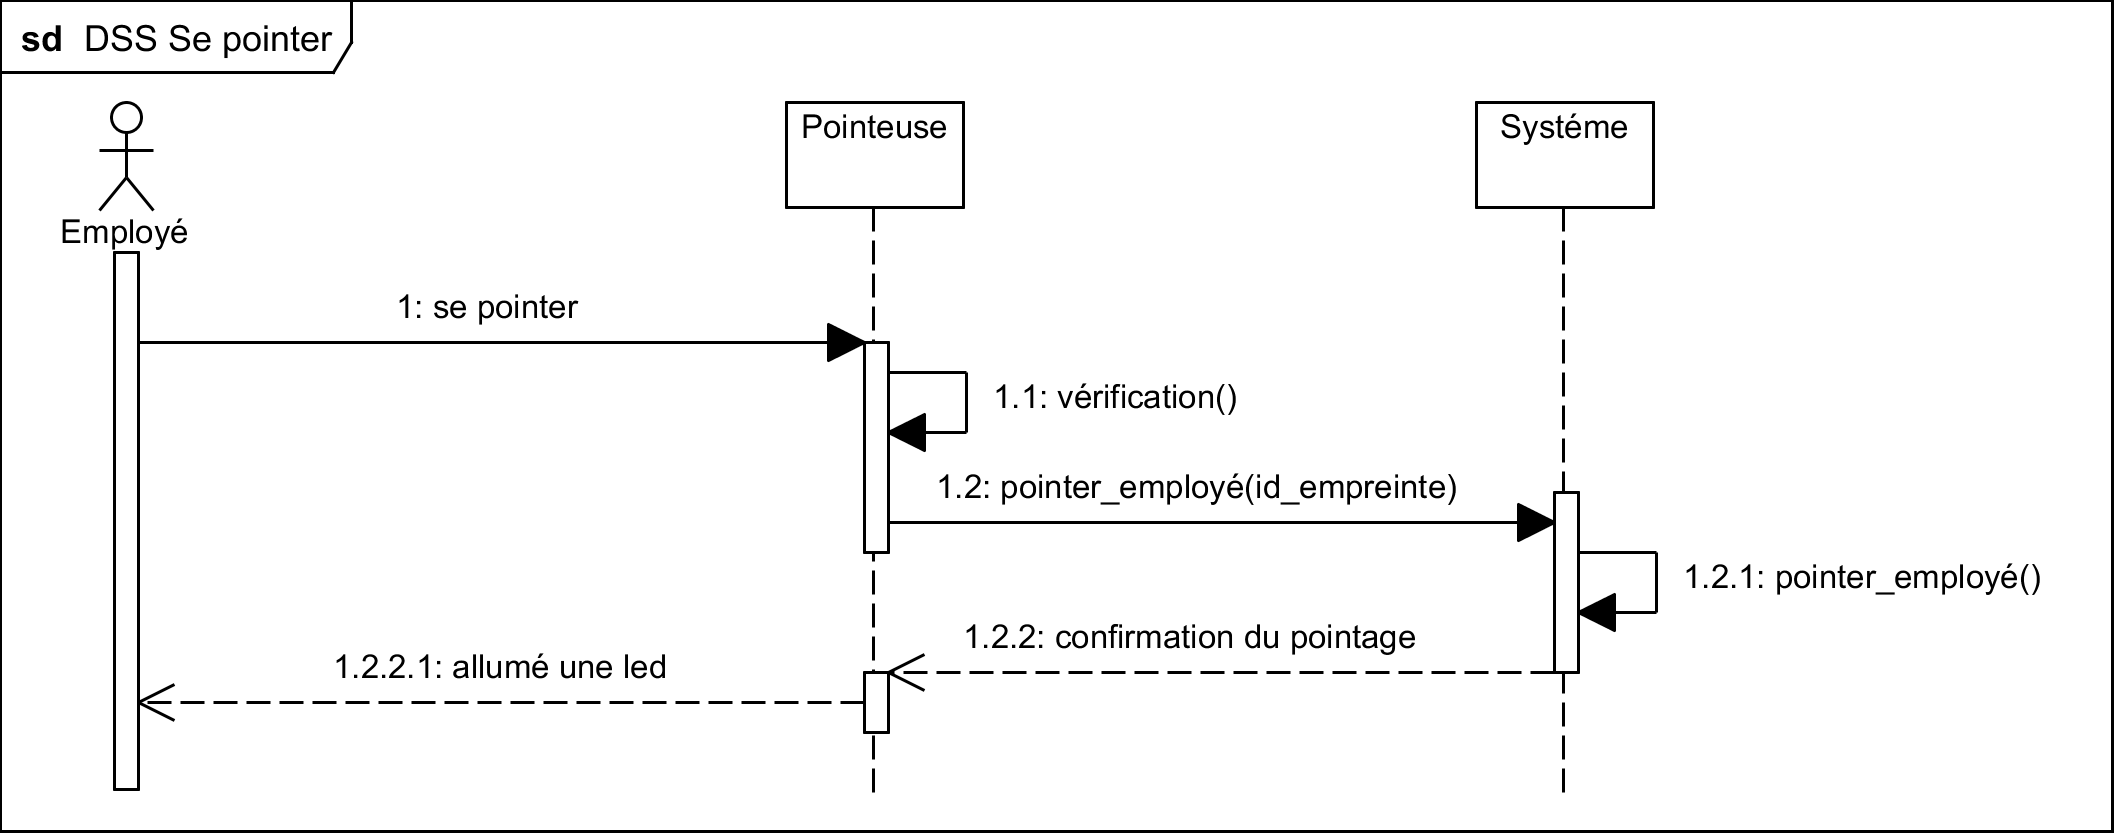
\includegraphics[scale=0.9]{images/DSS/DSS Se pointer.png}
         \caption{Diagramme de séquence système « Se pointer »}
         \label{fig4}
    \end{figure}
\vspace{-30pt}

\subsection{Cas d'utilisation « Consulter mon profil »}
L’employé peut décider de consulter son profil et avoir accès aux différentes
informations qui le concernent et modifier certaines valeurs s’il le souhaite, 
ou accéder à son planning. 
 
\begin{figure}[h!]
     \centering
     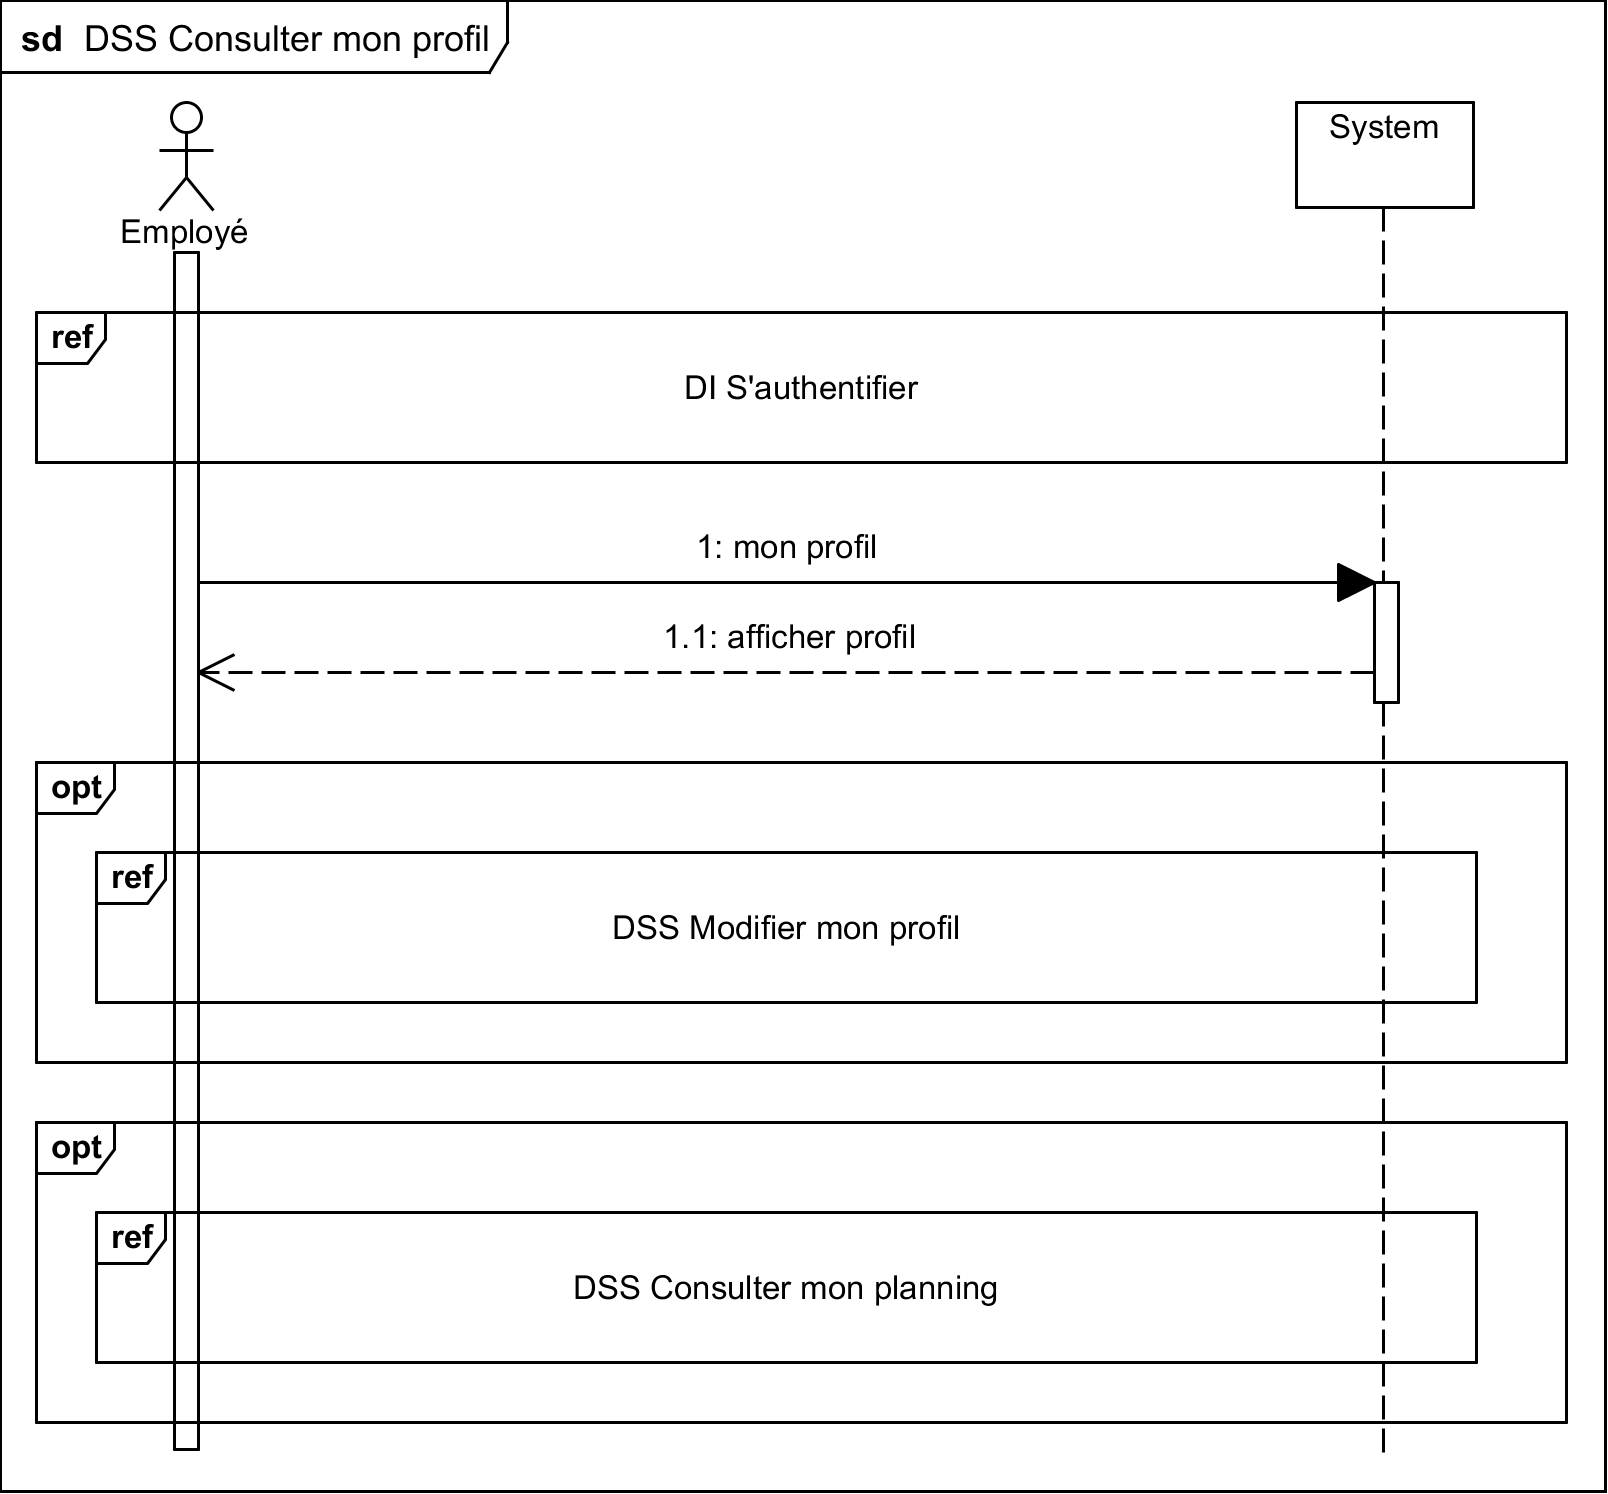
\includegraphics[scale=0.9]{images/DSS/DSS Consulter mon profil.png}
     \caption{Diagramme de séquence système « Consulter mon profil »}
     \label{fig4}
\end{figure}

\subsection{Cas d'utilisation « Consulter ma  fiche de pointage »}
Un employé peut consulter sa propre fiche de pointage qui comporte toutes les
informations concernant ses heures d’arrivée et de sortie des jours précédents.
Il peut aussi avoir a un affichage par semaine ou par mois.
   
\begin{figure}[h!]
     \centering
     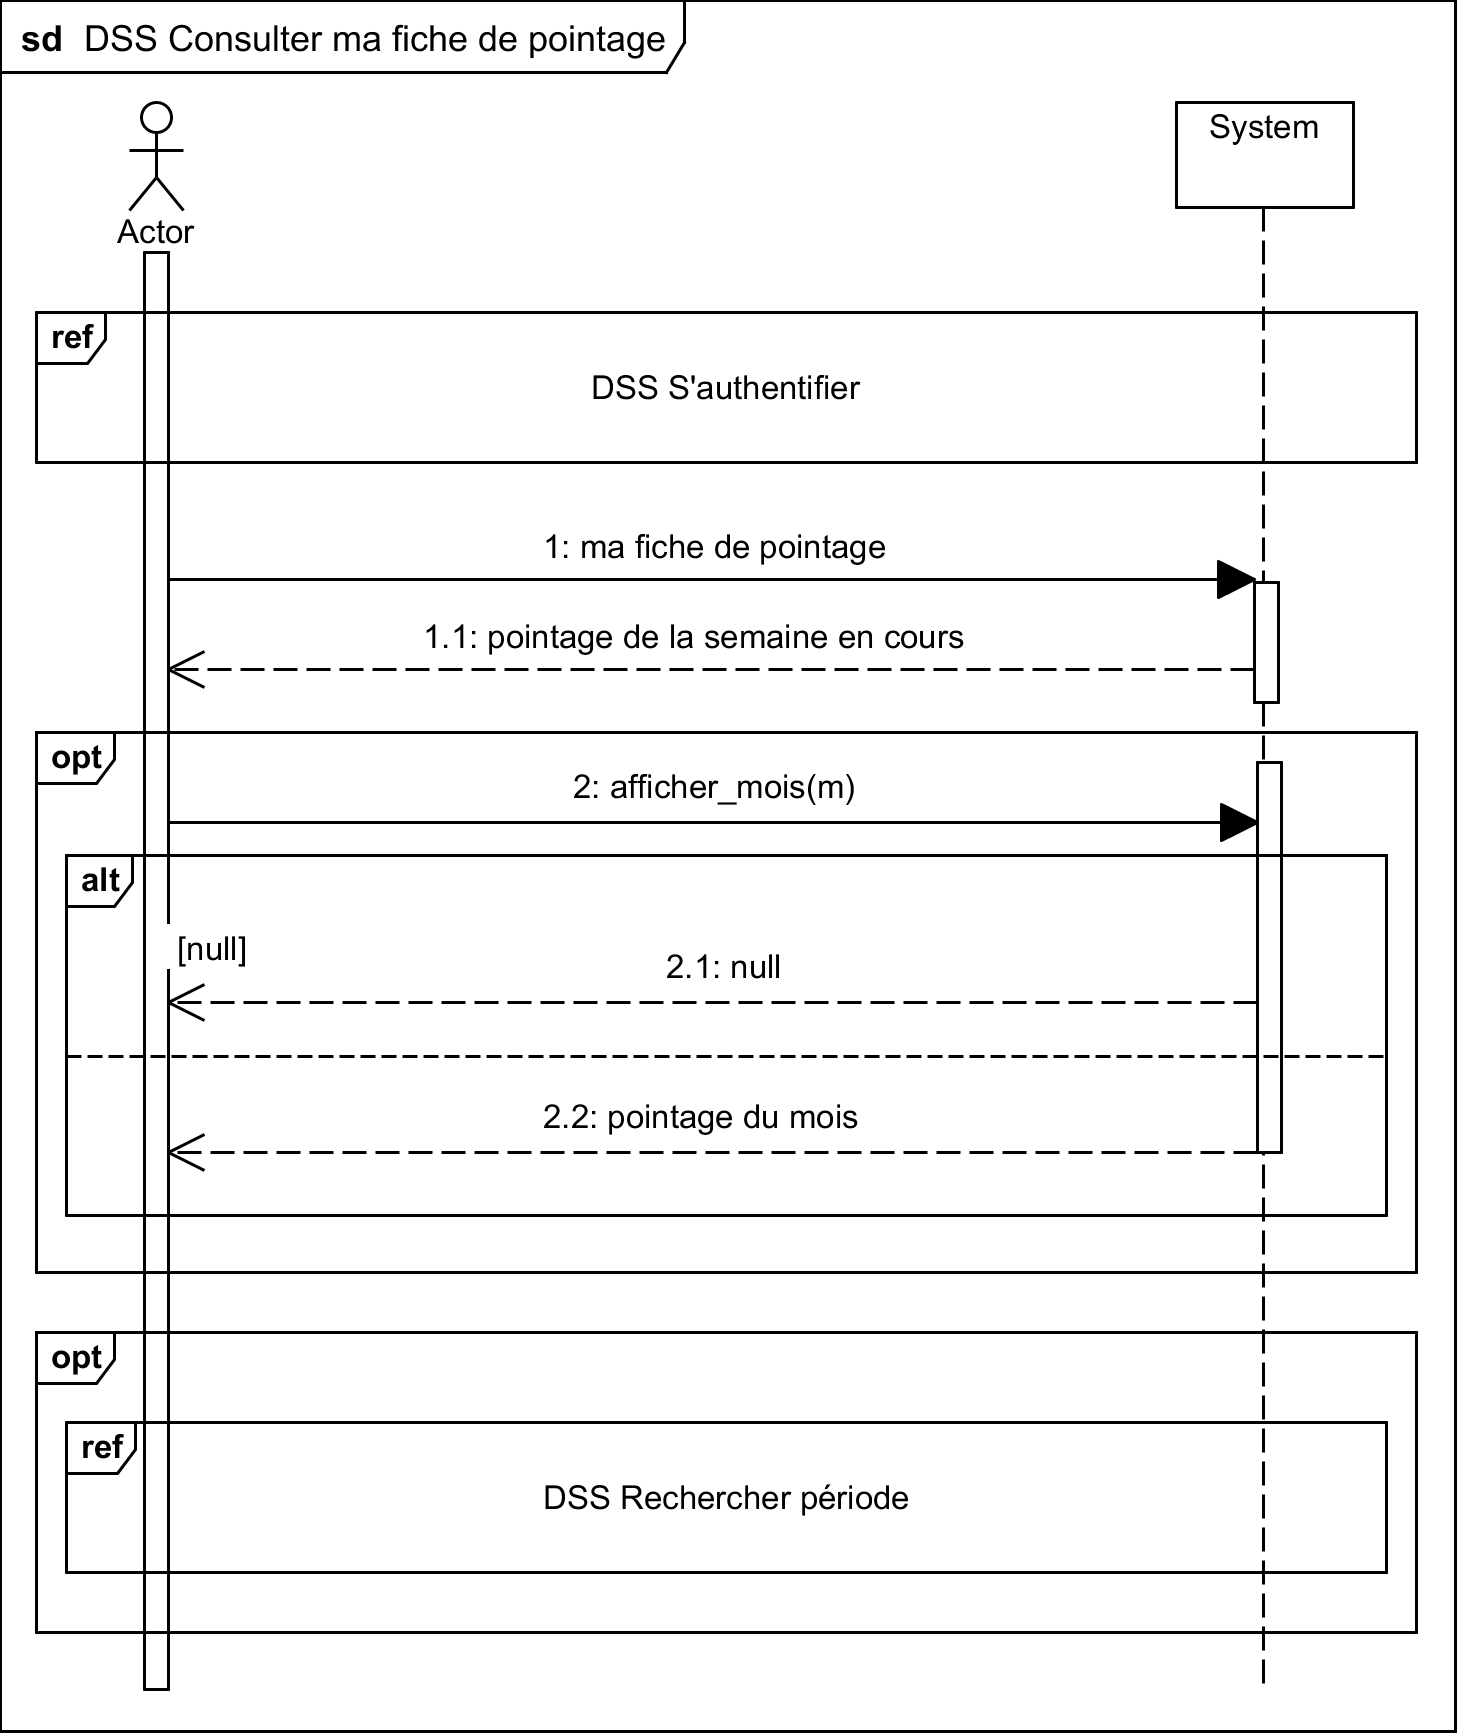
\includegraphics[scale=1.1]{images/DSS/DSS Consulter ma fiche de pointage.png}
     \caption{Diagramme de séquence système « Consulter ma  fiche de pointage »}
     \label{fig4}
\end{figure}

\vspace{-30pt}
\subsection{Cas d'utilisation « Consulter tableau de bord manager »}
Une fois authentifié, le manager sera redirigé directement vers son tableau de
bord qui est composé d’un espace en tant qu’employé et d'un autre consacré à ses
équipes. Grâce auquel il aura un récapitulatif de présence de ses
collaborateurs, leurs nombres, ainsi que leur dernier pointage et le temps passé
en poste.

\begin{figure}[h!]
     \centering
    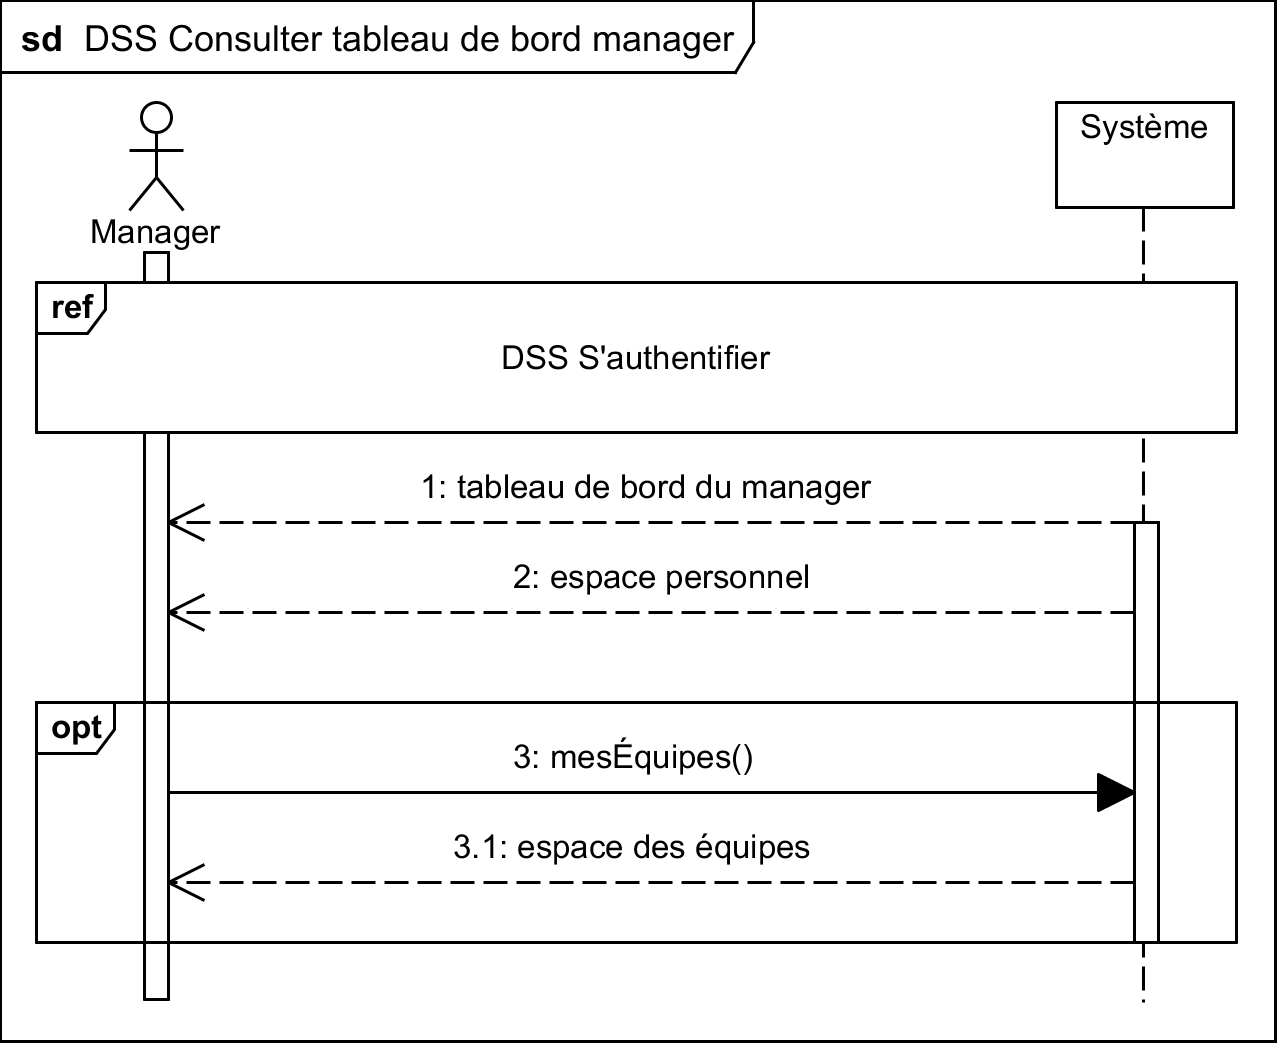
\includegraphics[scale=1]{images/DSS/DSS Consulter tableau de bord manager.png}
     \caption{Diagramme de séquence système « Consulter tableau de bord manager »}
     \label{fig4}
\end{figure}

\vspace{-30pt}
\subsection{Cas d'utilisation « Ajouter membre »}
Un responsable décide d’ajouter un membre à une équipe, il commence par
sélectionner l’équipe puis il effectue une recherche pour trouver l’employé pour
enfin l’ajouter en tant que membre de cette dernière.  

\begin{figure}[h!]
     \centering
    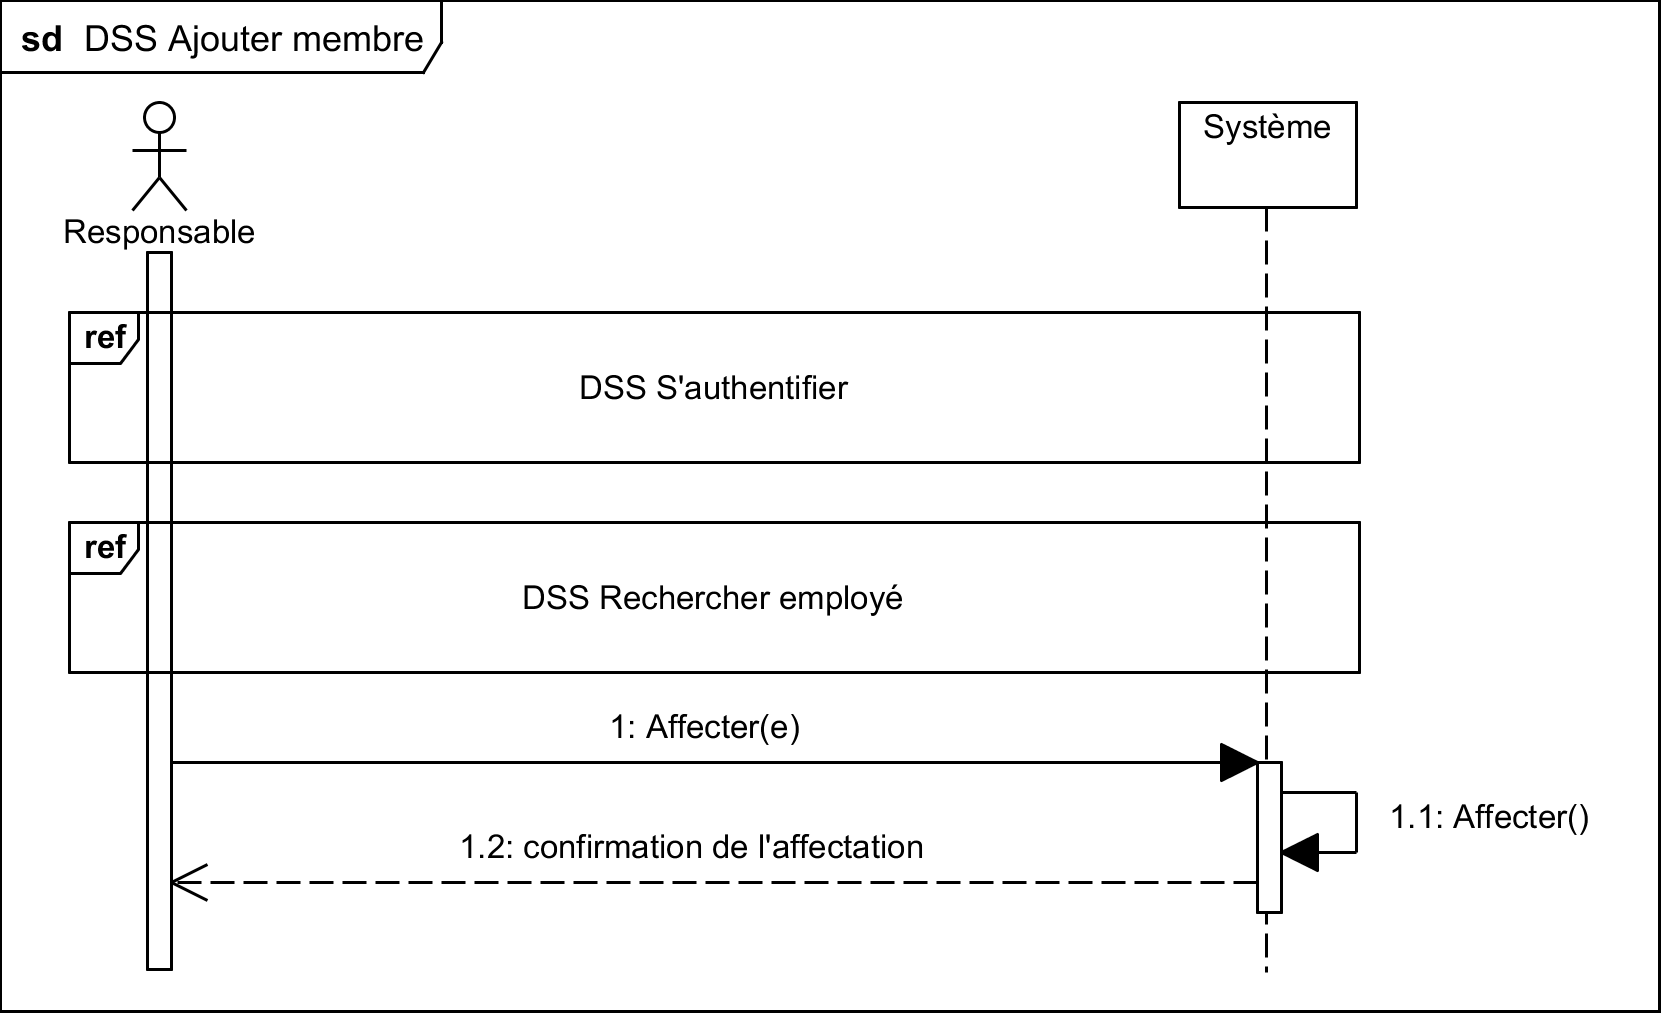
\includegraphics[scale=1]{images/DSS/DSS Ajouter membre.png}
     \caption{Diagramme de séquence système « Ajouter membre »}
     \label{fig4}
\end{figure}
    
\subsection{Cas d'utilisation « Ajouter planning »}
Un responsable peut créer un planning d’une semaine où il définit les jours de
travail ainsi que les horaires pour chaque jour. Pour ce, il doit saisir un
intitulé pour le planning et une description ainsi que les horaires d’entrée et
de sortie.   

\begin{figure}[h!]
     \centering
    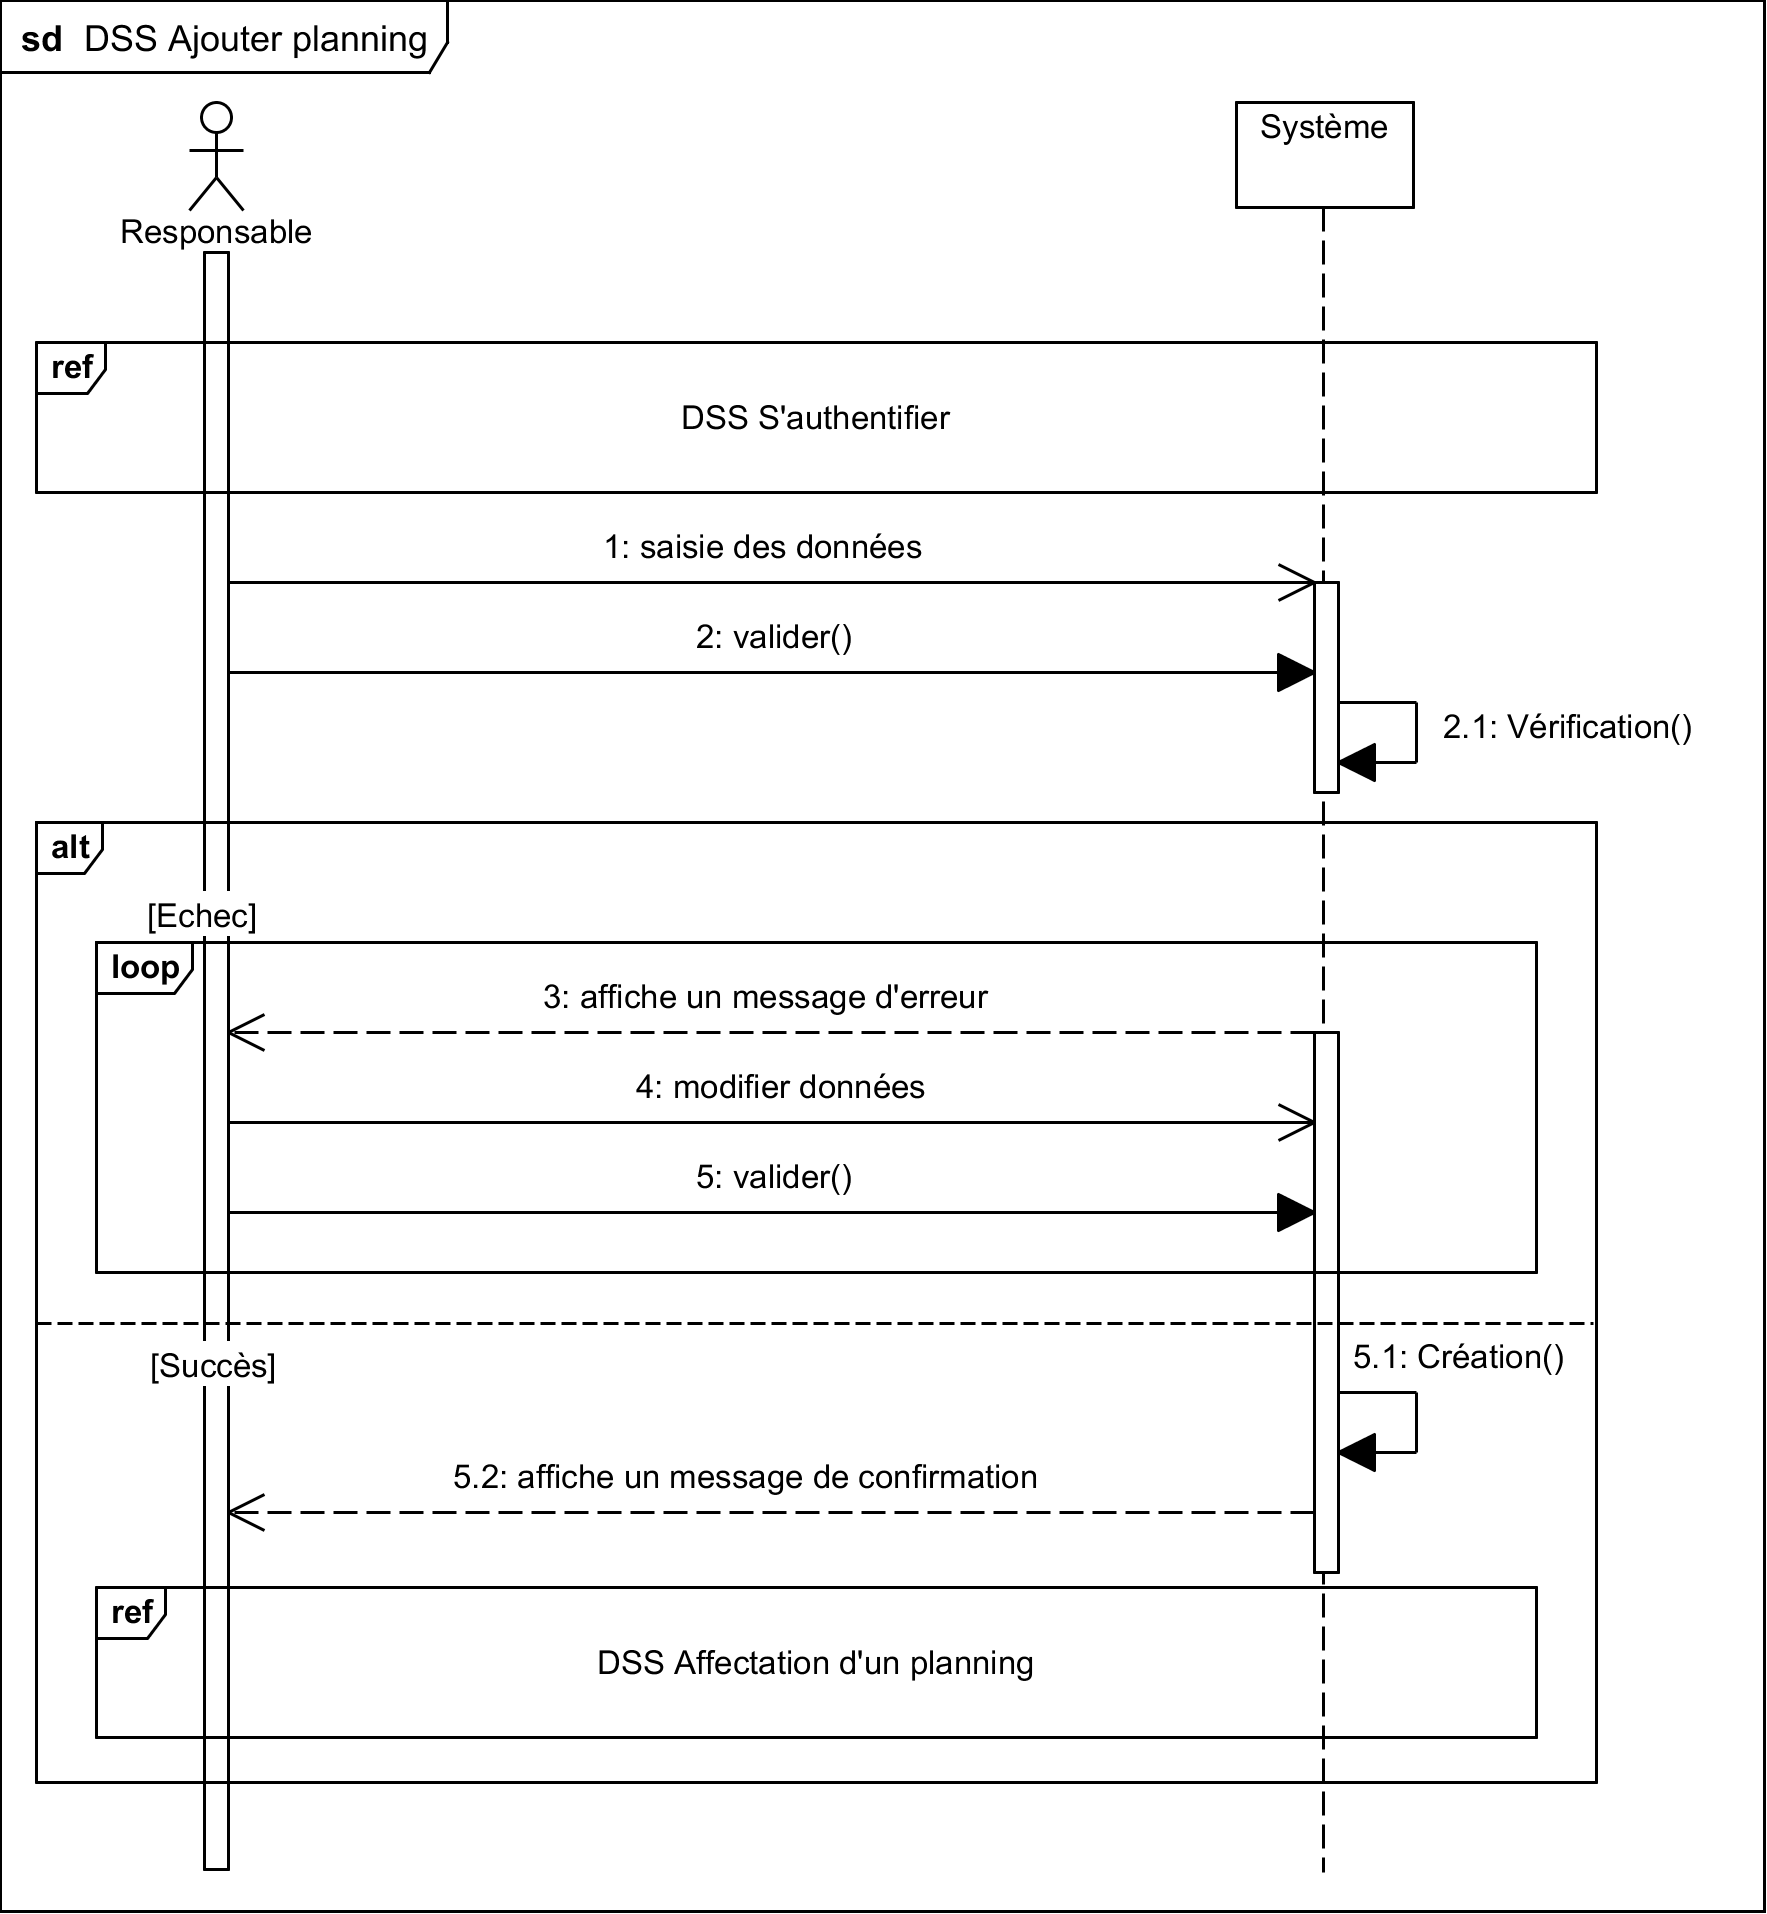
\includegraphics[scale=1]{images/DSS/DSS Ajouter planning.png}
     \caption{Diagramme de séquence système « Ajouter planning »}
     \label{fig4}
\end{figure}
    
\subsection{Cas d'utilisation « Ajouter équipe »}
Pour créer une équipe, le responsable doit saisir l’intitulé et la description
de l’équipe puis lui attribuer un manager. Une fois l’équipe créée, il pourra
ajouter des membres à cette équipe.   

\clearpage
\begin{figure}[h!]
     \centering
    \includegraphics[scale=1]{images/DSS/DSS Ajouter une équipe.png}
     \caption{Diagramme de séquence système « Ajouter équipe »}
     \label{fig4}
\end{figure}
    
\subsection{Cas d'utilisation « Ajouter employé »}
Un responsable peut créer un employé, il doit saisir les informations le
concernant. Une fois l’employé crée, il doit ajouter son empreinte.   

\clearpage
\begin{figure}[h!]
     \centering
    \includegraphics[scale=1.1]{images/DSS/DSS Ajouter employé.png}
     \caption{Diagramme de séquence système « Ajouter employé »}
     \label{fig4}
\end{figure}

\subsection{Cas d'utilisation « Consulter le profil d'un employé »}
Le responsable peut consulter le profil d’un employé qui contient les
informations de ce dernier. Il aura aussi la possibilité de le modifier ainsi
que de consulter son planning.

\clearpage
\begin{figure}[h!]
     \centering
    \includegraphics[scale=1]{images/DSS/DSS Consulter profil d'un employé.png}
     \caption{Diagramme de séquence système « Consulter profil d'un employé »}
     \label{fig4}
\end{figure}

Dans un souci de lisibilité, nous avons déplacé le reste des diagrammes de
séquence système vers l’annexe B \ref{ch:annexeB}.  
    
\section{Les maquettes IHM }
    
\subsection{Employé}
La figure \ref{fig6} : Une fois, authentifié, cette interface sera la première
affichée à l’utilisateur ayant le rôle d’un employé. On remarque un menu sur le
côté gauche, un composant qui sera présent sur la totalité des interfaces du
projet, et qui permet une navigation entre les différentes fonctionnalités
qu’offre le système tout en s’adaptant au rôle de l’utilisateur connecté.
L’utilisateur peut à tout moment se déconnecter grâce au bouton présent au bas
du menu.

Cette interface représente le tableau de bord de l’employé, elle regroupe les
informations les plus récentes et les plus pertinentes, comme ses horaires du
jour ou son dernier pointage ainsi que le temps passé en poste. Une seconde
partie est dédiée à des informations concernant ses collaborateurs faisant
partie de son équipe.
        
La figure \ref{fig7} : représente l’affichage du profil de l’employé lui-même,
où ses informations sont regroupées en catégories selon leurs utilité et leurs
importance. Il existe un bouton qui permet à l’employé de visualiser son
planning à partir de cette interface directement. 

\clearpage
        
\begin{figure}[h!]
    \centering
    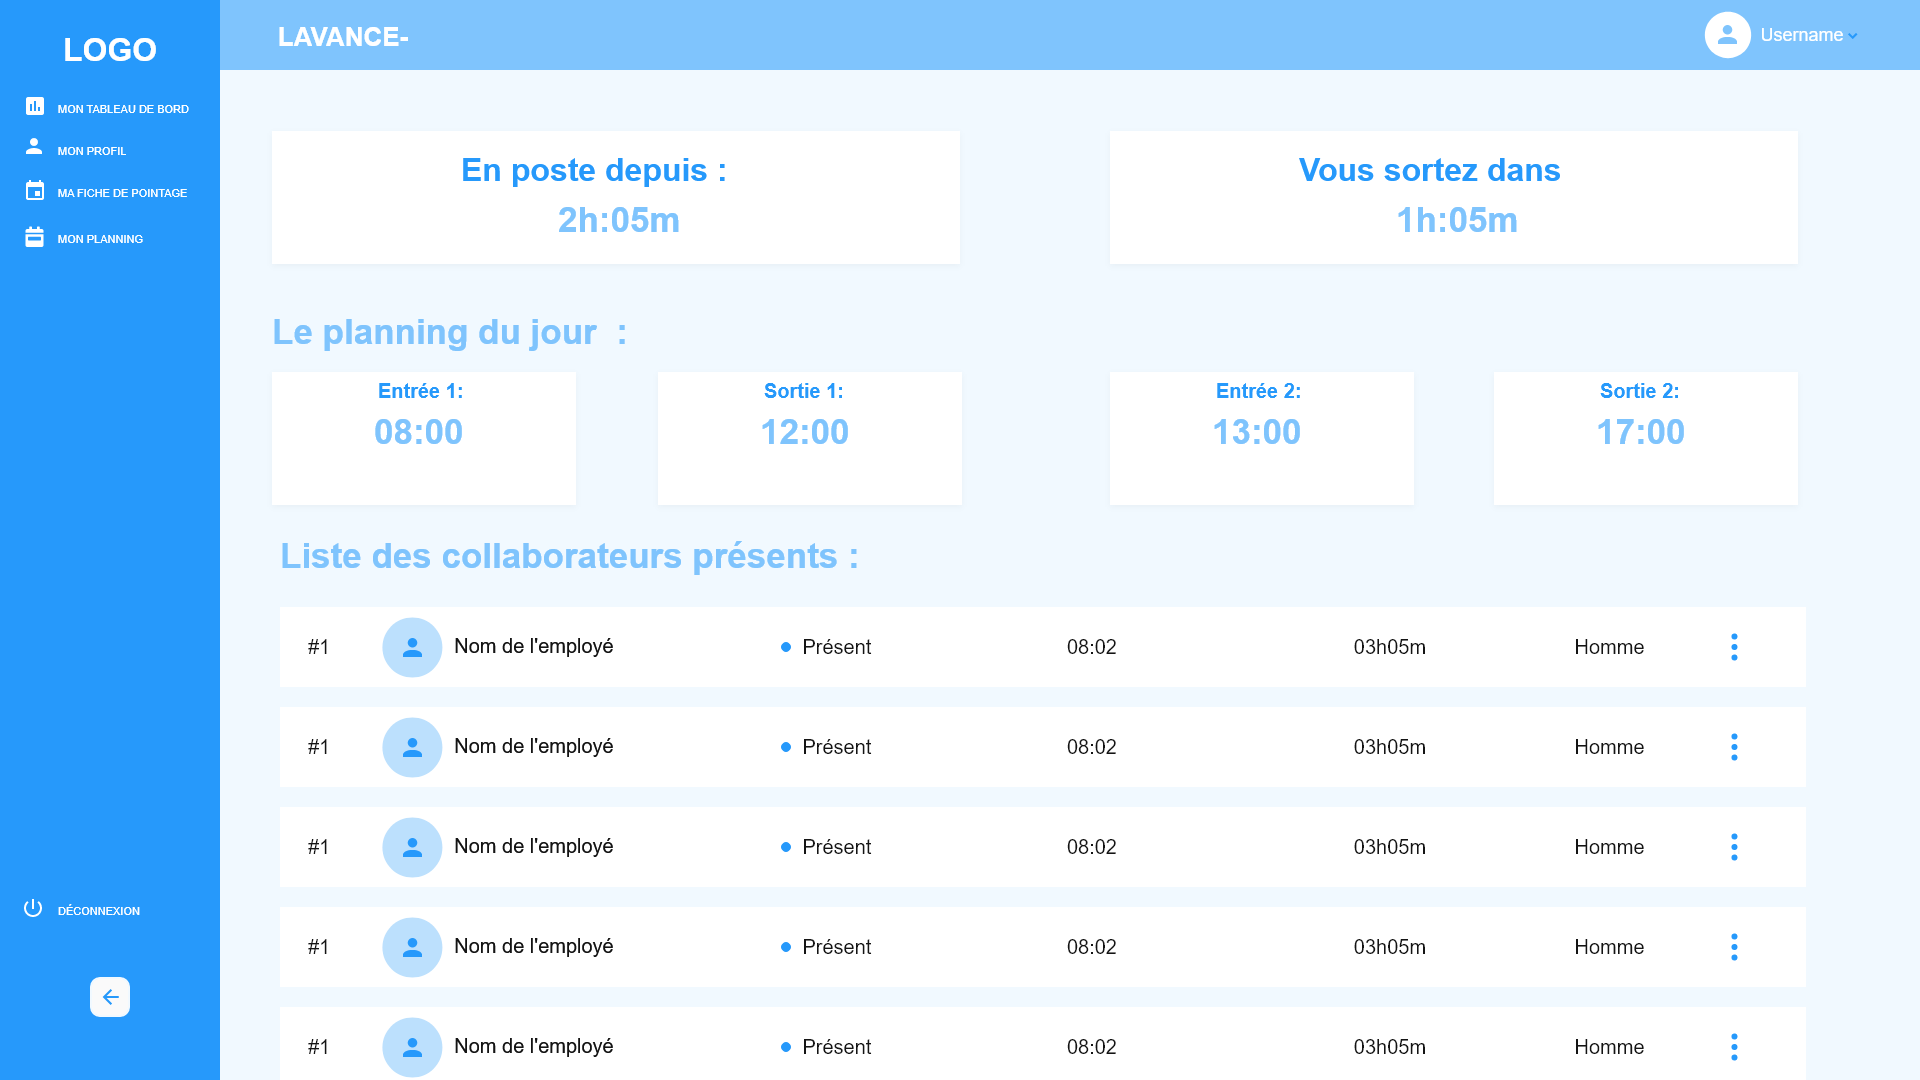
\includegraphics[width=18cm]{images/dash_emp.png}
    \caption{Maquette tableau de bord Employé}
    \label{fig6}
\end{figure}

\begin{figure}[h!]
    \centering
    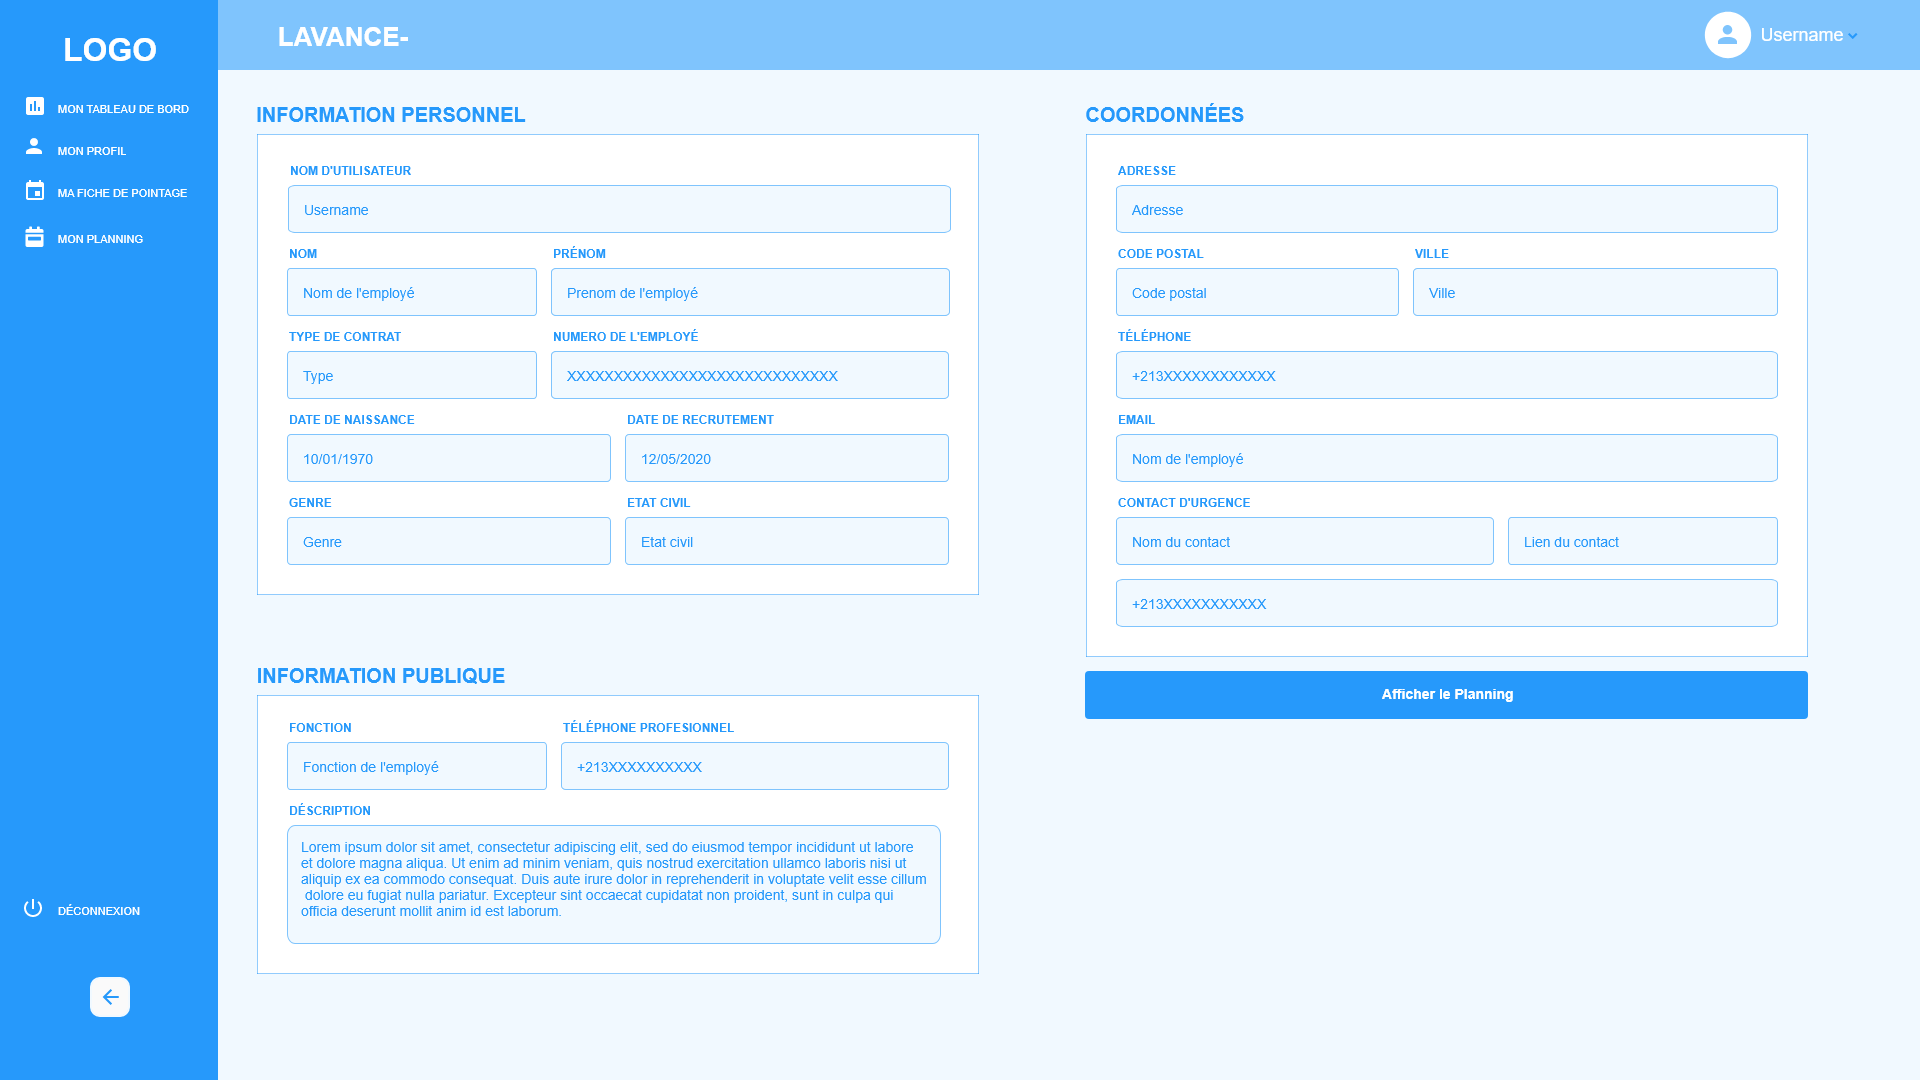
\includegraphics[width=18cm]{images/profil.png}
    \caption{Maquette profil Employé}
    \label{fig7}    
\end{figure}
        
\subsection{Manager}
La figure \ref{fig8} : ici, on représente le tableau de bord du manager qui est
composé de deux onglets. Le premier onglet est identique au tableau de bord de
l’employé simple, tandis que l’onglet « Mes équipes » récapitule l’ensemble des
informations concernant les équipes sous la responsabilité d’un manager. Il met
en évidence le nombre total des équipes et des collaborateurs, le récapitulatif
de présence de ces derniers sous forme de graphe, ainsi qu’une liste des
employés avec leurs derniers pointages
        
La figure \ref{fig9} : cette interface affiche les informations qui concernent
une équipe sélectionnée au préalable par le manager. On peut y voir le titre, la
description de l’équipe ainsi que des statistiques. Dans la partie inférieure,
on liste l’ensemble des employés appartenant à cette équipe avec la possibilité
d’un accès direct vers le profil de chacun d’eux.

\begin{figure}[h!]
    \centering
    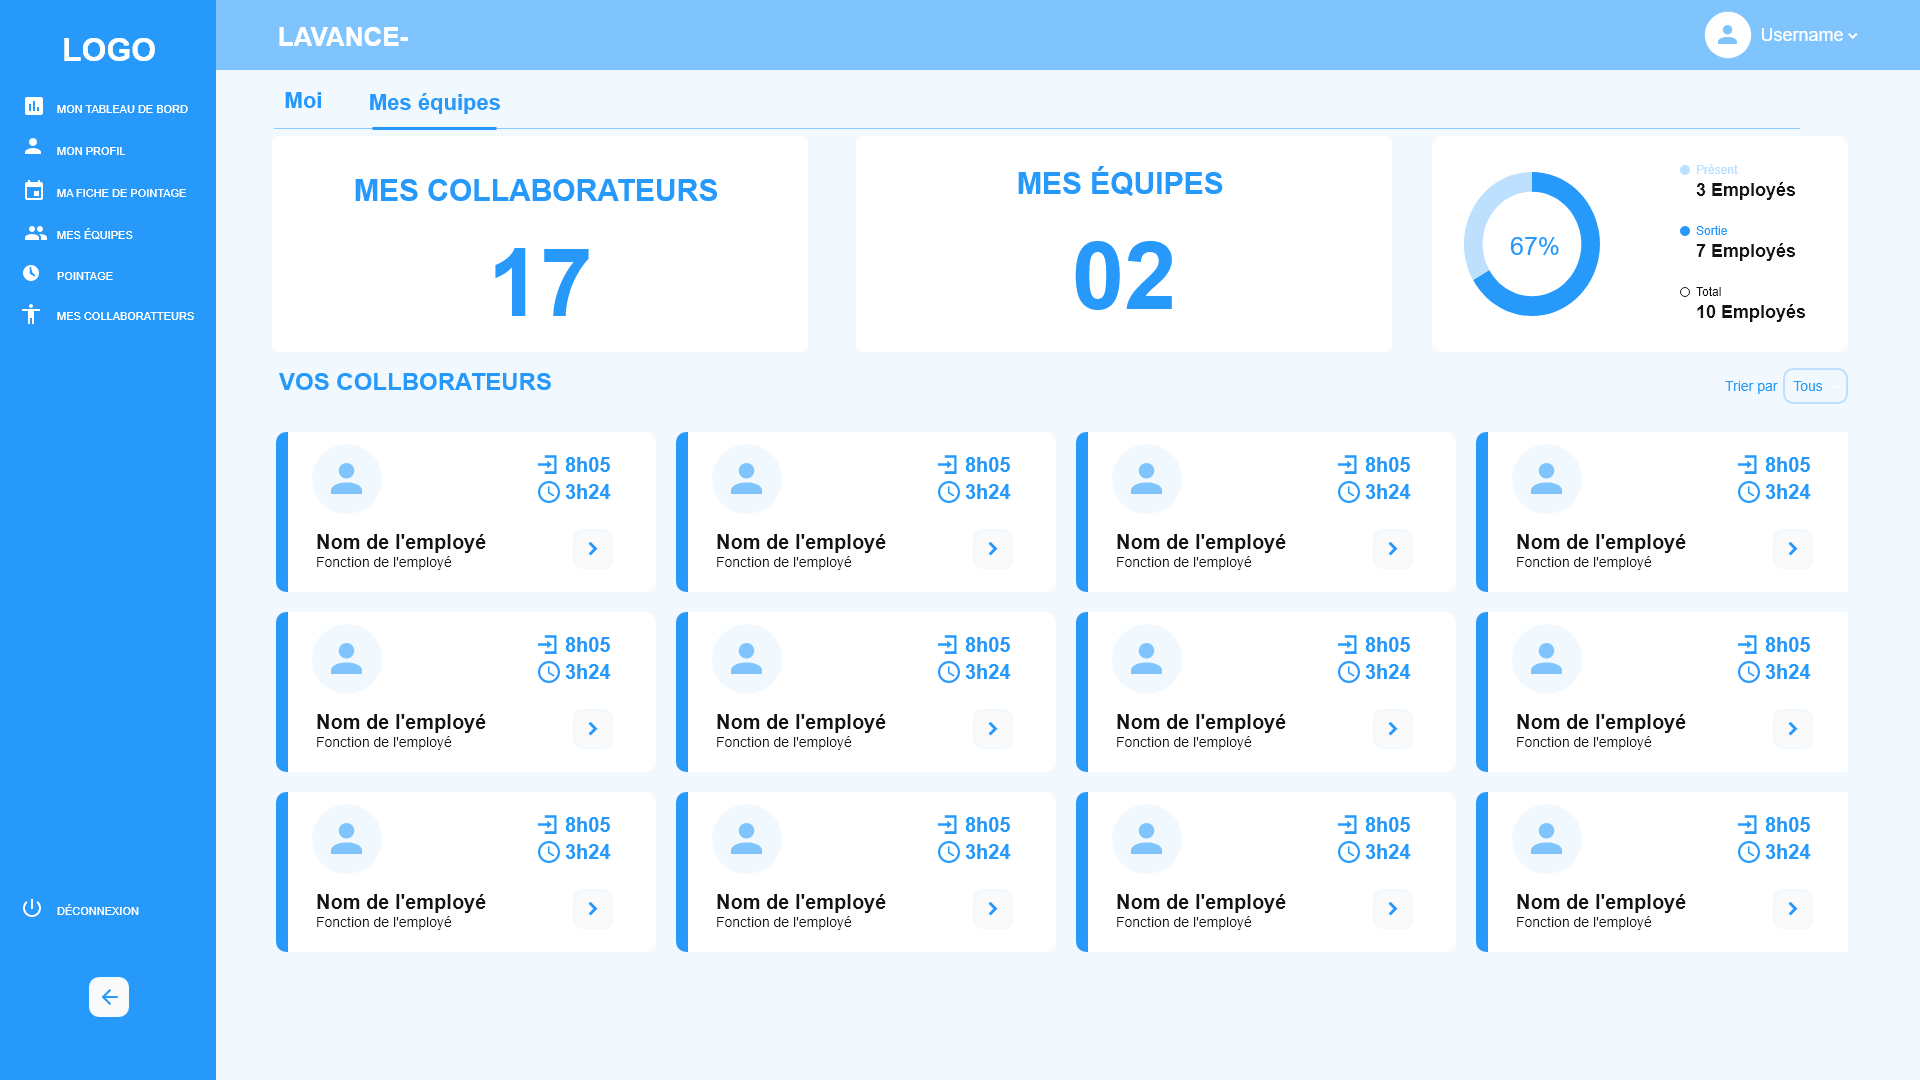
\includegraphics[width=18cm]{images/dash_man_my_teams.png}
    \caption{Maquette tableau de bord Manager}
    \label{fig8}
\end{figure}

\clearpage

\begin{figure}[h!]
    \centering
    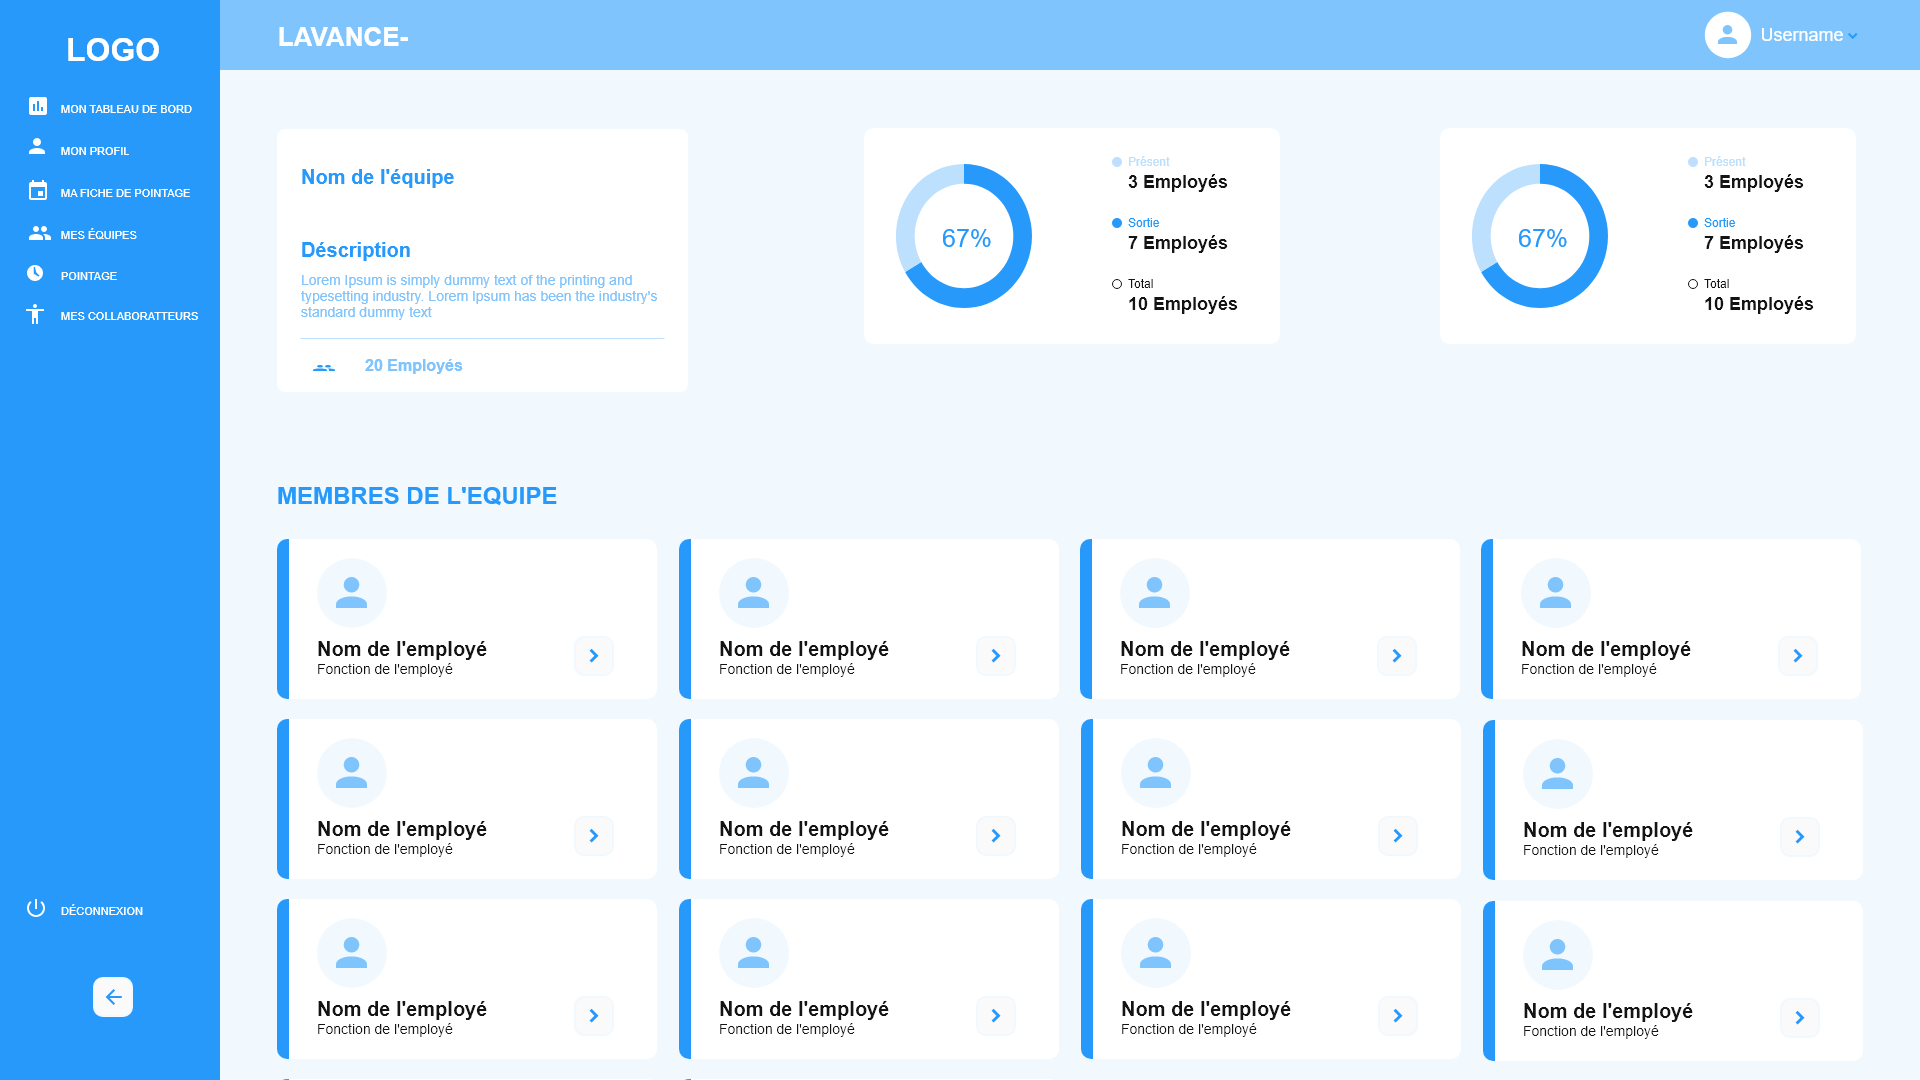
\includegraphics[width=18cm]{images/my_team.png}
    \caption{Maquette les équipes d'un Manager}
    \label{fig9}
\end{figure}


\subsection{Responsable}
La figure \ref{fig10} : représente l’interface dans laquelle le responsable crée
un planning en lui attribuant un nom et une description et les horaires de début
et de fin des périodes de travail tout au long de la semaine, avec chaque jour
étant composé de deux parties.
 
La figure \ref{fig11} : représente l’interface avec laquelle un responsable
affecte un planning à un ou des employés en effectuant une recherche par lettre
qui affiche une liste des employés ayant un nom ou un prénom correspondant aux
caractères saisis, et un bouton qui permet d’affecter l’employé sélectionné.
L’interface comporte aussi une liste des employés ayant déjà été affectés à ce
planning avec la possibilité de détacher un employé du planning. 

\clearpage

\begin{figure}[h!]
    \centering
    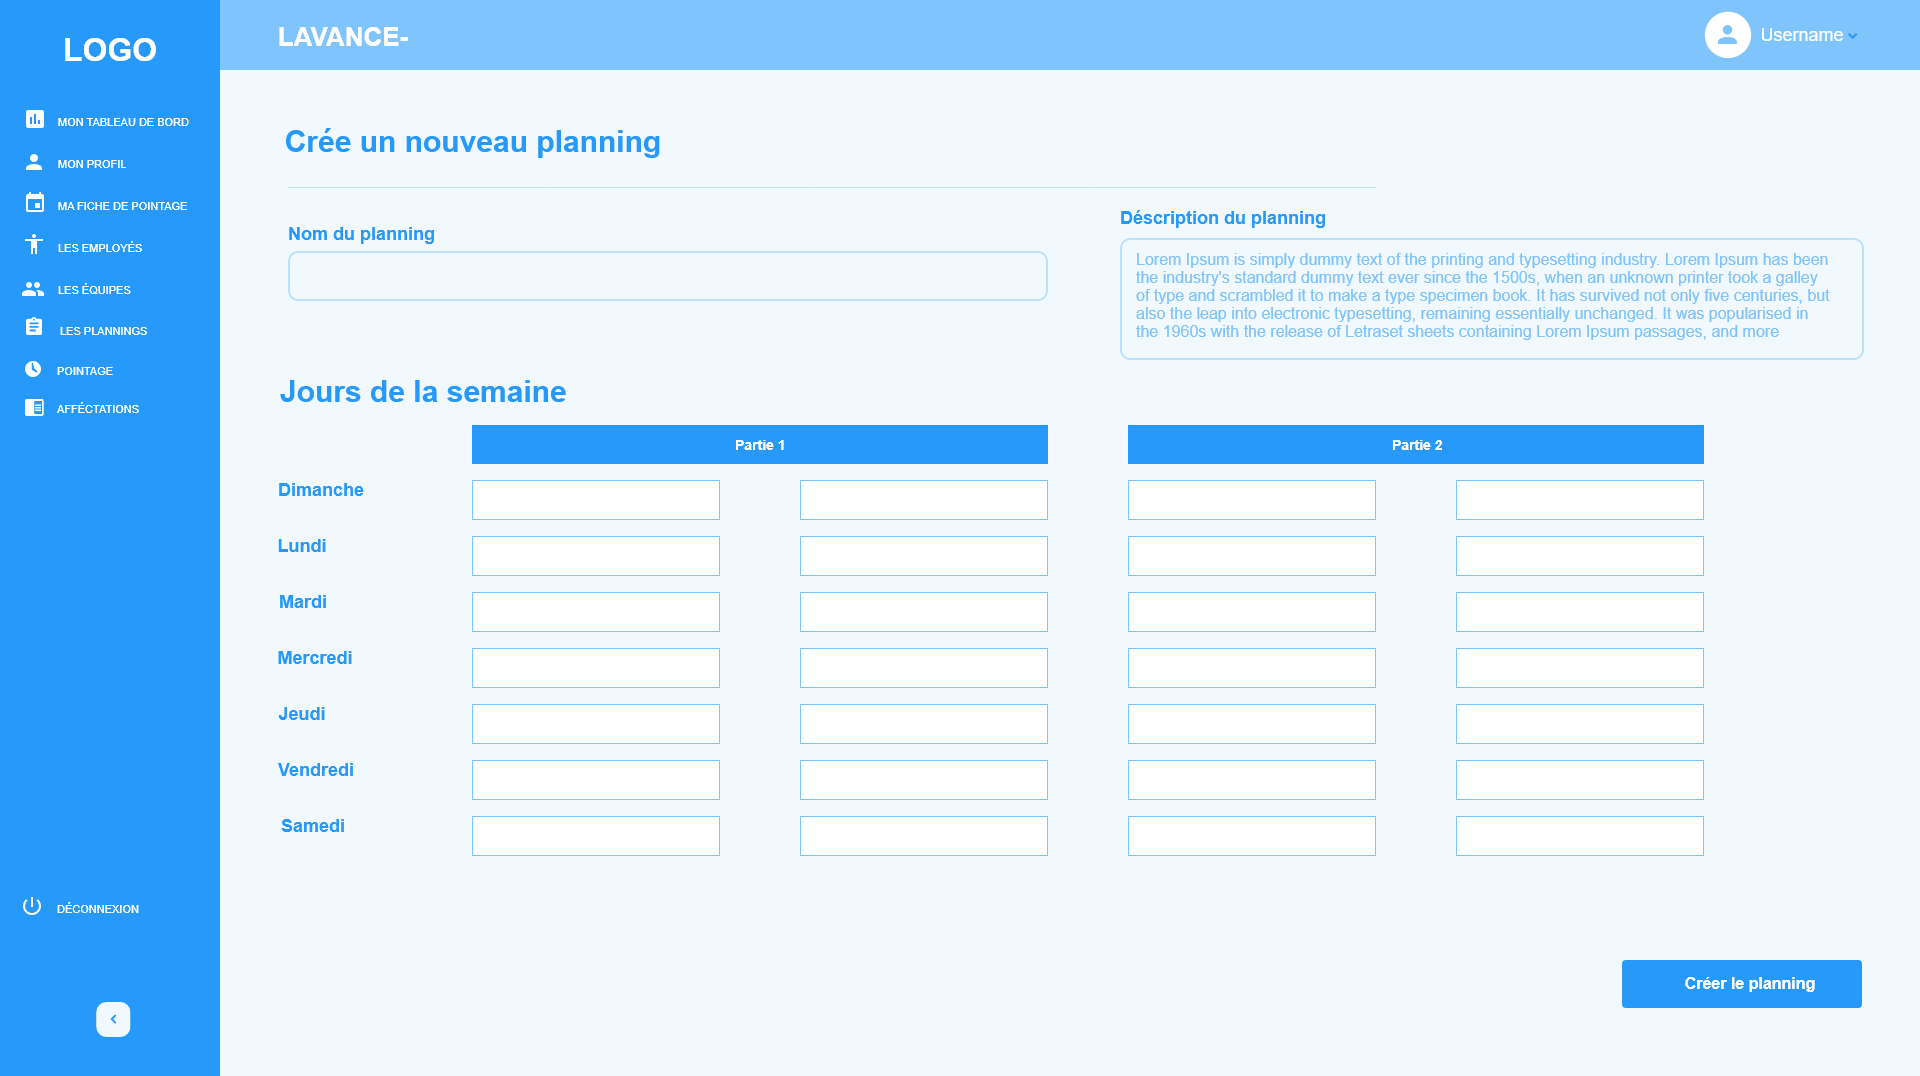
\includegraphics[width=18cm]{images/add_panning.png}
    \caption{Maquette création d'un planning}
    \label{fig10}
\end{figure}



\begin{figure}[h!]
    \centering
    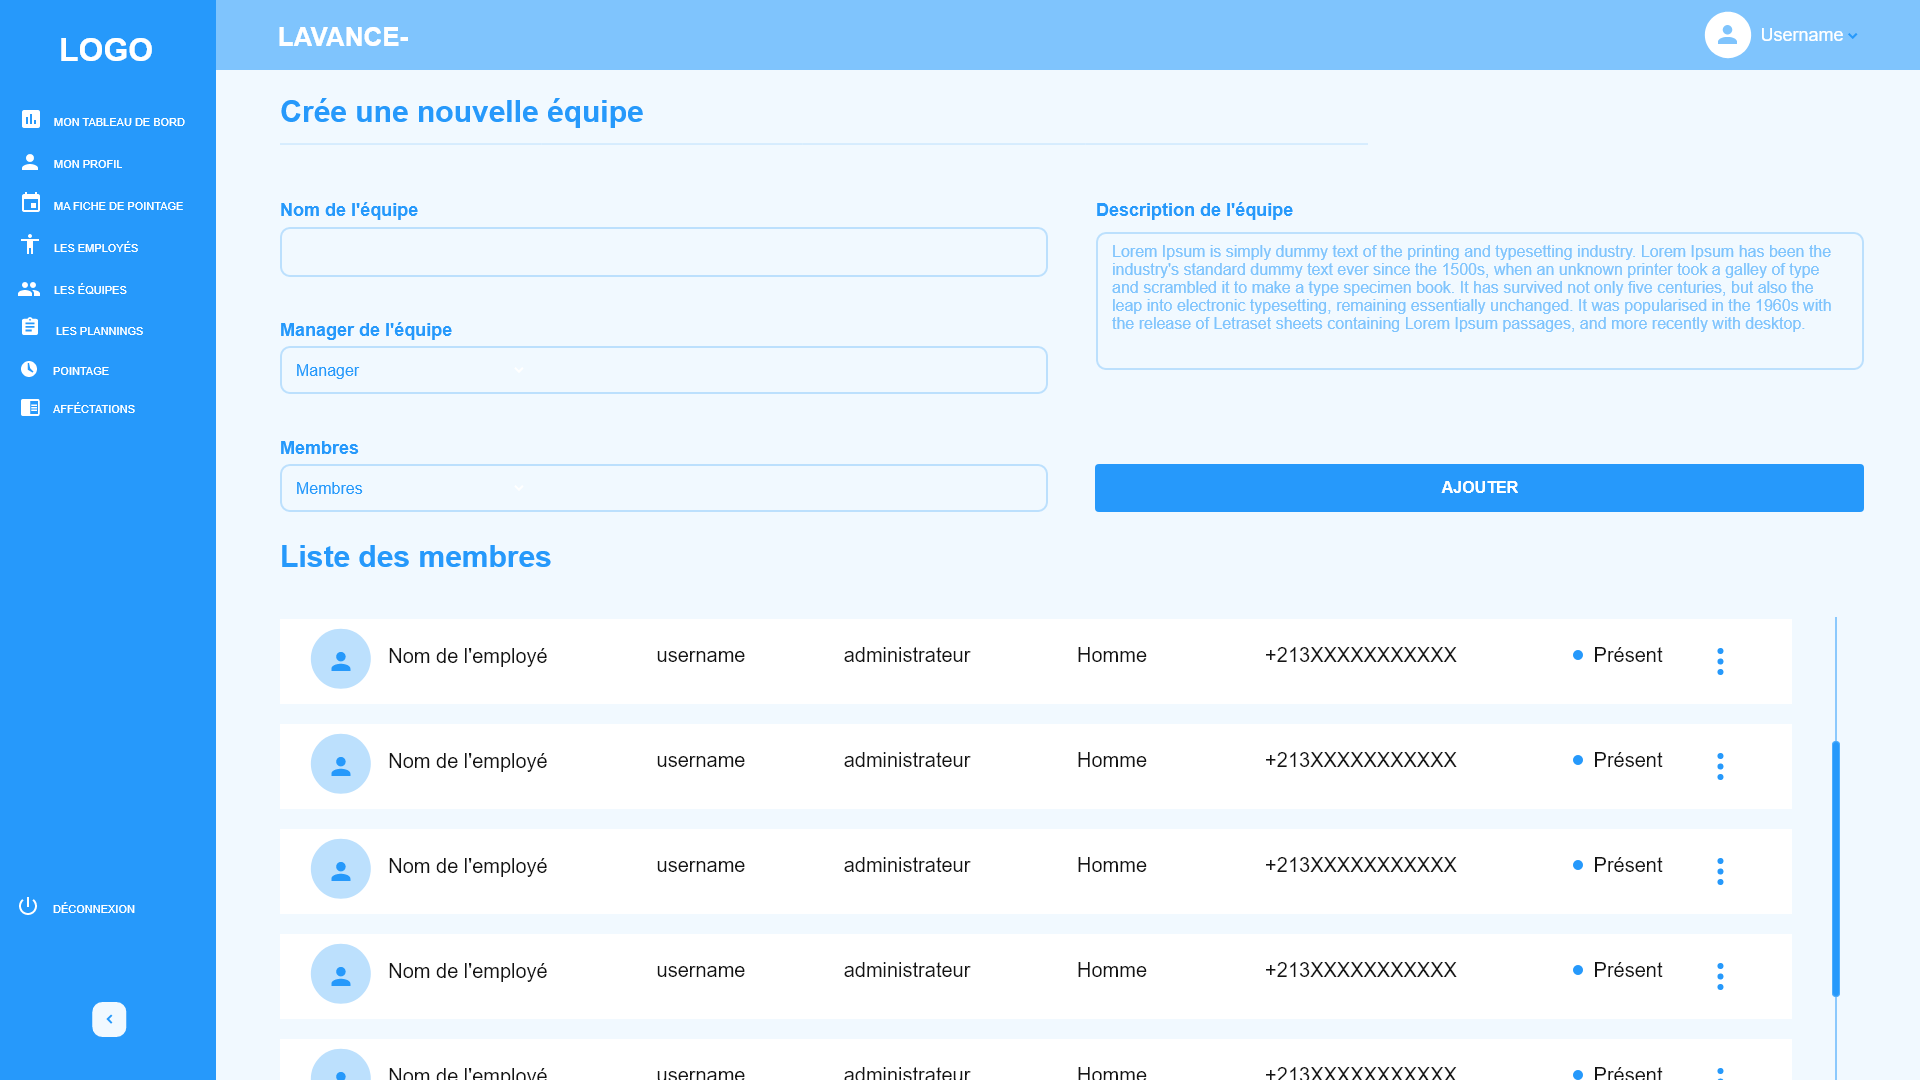
\includegraphics[width=18cm]{images/add_member.png}
    \caption{Maquette affectations d'un employé a une équipe }
    \label{fig11}
\end{figure}

\clearpage
À travers ces quelques maquettes, nous avons essayé de vous transmettre notre
vision générale du projet sur son aspect graphique, et la composition globale de
certaines interfaces. Le reste des maquettes sera présenté de manière détaillée
dans l’annexe.
        
\subsection{la navigation}
L’outil utilisé pour réaliser les maquettes offre la possibilité de créer un
prototype complet et très représentatif du résultat final. Ci-dessous, des liens
vers les prototypes réalisés comportant toutes les interfaces et les liens de
navigations.\\

Prototype employé: \href{https://xd.adobe.com/view/9afd474c-7053-4831-4a92-bb9d2f4d8c65-eccc/?fullscreen&hints=off}{lien du prototype 1}
URL :<https://xd.adobe.com/view/9afd474c-7053-4831-4a92-bb9d2f4d8c65-eccc/?fullscreen&hints=off>\\
Prototype manager: \href{https://xd.adobe.com/view/855f8afc-8c35-451d-7b50-838460e72c7e-f36e/?fullscreen&hints=off}{lien du prototype 2}
URL :<https://xd.adobe.com/view/855f8afc-8c35-451d-7b50-838460e72c7e-f36e/?fullscreen&hints=off>\\
Prototype responsable: \href{https://xd.adobe.com/view/8c62407e-81ae-4950-60f2-88006b652695-fa53/?fullscreen&hints=off}{lien du prototype 3}
URL :<https://xd.adobe.com/view/8c62407e-81ae-4950-60f2-88006b652695-fa53/?fullscreen&hints=off>

        
\section{Conclusion}
Ce chapitre nous a permis d’exprimer et d’analyser les besoins permettant de
décrire les fonctionnalités du système de manière globale. Aussi, grâce à
l’identification des acteurs et des cas d’utilisations, nous avons formalisé les
différents besoins fonctionnels et non fonctionnels, défini les digrammes de cas
d’utilisations, réalisé les maquettes IHM et la navigation. Tout ceci nous
permettra, dans le chapitre suivant, de réaliser les différents modèles de la
phase de conception.
